% Options for packages loaded elsewhere
\PassOptionsToPackage{unicode}{hyperref}
\PassOptionsToPackage{hyphens}{url}
%
\documentclass[
]{book}
\usepackage{lmodern}
\usepackage{amssymb,amsmath}
\usepackage{ifxetex,ifluatex}
\ifnum 0\ifxetex 1\fi\ifluatex 1\fi=0 % if pdftex
  \usepackage[T1]{fontenc}
  \usepackage[utf8]{inputenc}
  \usepackage{textcomp} % provide euro and other symbols
\else % if luatex or xetex
  \usepackage{unicode-math}
  \defaultfontfeatures{Scale=MatchLowercase}
  \defaultfontfeatures[\rmfamily]{Ligatures=TeX,Scale=1}
\fi
% Use upquote if available, for straight quotes in verbatim environments
\IfFileExists{upquote.sty}{\usepackage{upquote}}{}
\IfFileExists{microtype.sty}{% use microtype if available
  \usepackage[]{microtype}
  \UseMicrotypeSet[protrusion]{basicmath} % disable protrusion for tt fonts
}{}
\makeatletter
\@ifundefined{KOMAClassName}{% if non-KOMA class
  \IfFileExists{parskip.sty}{%
    \usepackage{parskip}
  }{% else
    \setlength{\parindent}{0pt}
    \setlength{\parskip}{6pt plus 2pt minus 1pt}}
}{% if KOMA class
  \KOMAoptions{parskip=half}}
\makeatother
\usepackage{xcolor}
\IfFileExists{xurl.sty}{\usepackage{xurl}}{} % add URL line breaks if available
\IfFileExists{bookmark.sty}{\usepackage{bookmark}}{\usepackage{hyperref}}
\hypersetup{
  pdftitle={Tests statistiques, la suite \ldots{}},
  pdfauthor={Cathy Maugis-Rabusseau (INSA Toulouse / IMT)},
  hidelinks,
  pdfcreator={LaTeX via pandoc}}
\urlstyle{same} % disable monospaced font for URLs
\usepackage{color}
\usepackage{fancyvrb}
\newcommand{\VerbBar}{|}
\newcommand{\VERB}{\Verb[commandchars=\\\{\}]}
\DefineVerbatimEnvironment{Highlighting}{Verbatim}{commandchars=\\\{\}}
% Add ',fontsize=\small' for more characters per line
\usepackage{framed}
\definecolor{shadecolor}{RGB}{248,248,248}
\newenvironment{Shaded}{\begin{snugshade}}{\end{snugshade}}
\newcommand{\AlertTok}[1]{\textcolor[rgb]{0.94,0.16,0.16}{#1}}
\newcommand{\AnnotationTok}[1]{\textcolor[rgb]{0.56,0.35,0.01}{\textbf{\textit{#1}}}}
\newcommand{\AttributeTok}[1]{\textcolor[rgb]{0.77,0.63,0.00}{#1}}
\newcommand{\BaseNTok}[1]{\textcolor[rgb]{0.00,0.00,0.81}{#1}}
\newcommand{\BuiltInTok}[1]{#1}
\newcommand{\CharTok}[1]{\textcolor[rgb]{0.31,0.60,0.02}{#1}}
\newcommand{\CommentTok}[1]{\textcolor[rgb]{0.56,0.35,0.01}{\textit{#1}}}
\newcommand{\CommentVarTok}[1]{\textcolor[rgb]{0.56,0.35,0.01}{\textbf{\textit{#1}}}}
\newcommand{\ConstantTok}[1]{\textcolor[rgb]{0.00,0.00,0.00}{#1}}
\newcommand{\ControlFlowTok}[1]{\textcolor[rgb]{0.13,0.29,0.53}{\textbf{#1}}}
\newcommand{\DataTypeTok}[1]{\textcolor[rgb]{0.13,0.29,0.53}{#1}}
\newcommand{\DecValTok}[1]{\textcolor[rgb]{0.00,0.00,0.81}{#1}}
\newcommand{\DocumentationTok}[1]{\textcolor[rgb]{0.56,0.35,0.01}{\textbf{\textit{#1}}}}
\newcommand{\ErrorTok}[1]{\textcolor[rgb]{0.64,0.00,0.00}{\textbf{#1}}}
\newcommand{\ExtensionTok}[1]{#1}
\newcommand{\FloatTok}[1]{\textcolor[rgb]{0.00,0.00,0.81}{#1}}
\newcommand{\FunctionTok}[1]{\textcolor[rgb]{0.00,0.00,0.00}{#1}}
\newcommand{\ImportTok}[1]{#1}
\newcommand{\InformationTok}[1]{\textcolor[rgb]{0.56,0.35,0.01}{\textbf{\textit{#1}}}}
\newcommand{\KeywordTok}[1]{\textcolor[rgb]{0.13,0.29,0.53}{\textbf{#1}}}
\newcommand{\NormalTok}[1]{#1}
\newcommand{\OperatorTok}[1]{\textcolor[rgb]{0.81,0.36,0.00}{\textbf{#1}}}
\newcommand{\OtherTok}[1]{\textcolor[rgb]{0.56,0.35,0.01}{#1}}
\newcommand{\PreprocessorTok}[1]{\textcolor[rgb]{0.56,0.35,0.01}{\textit{#1}}}
\newcommand{\RegionMarkerTok}[1]{#1}
\newcommand{\SpecialCharTok}[1]{\textcolor[rgb]{0.00,0.00,0.00}{#1}}
\newcommand{\SpecialStringTok}[1]{\textcolor[rgb]{0.31,0.60,0.02}{#1}}
\newcommand{\StringTok}[1]{\textcolor[rgb]{0.31,0.60,0.02}{#1}}
\newcommand{\VariableTok}[1]{\textcolor[rgb]{0.00,0.00,0.00}{#1}}
\newcommand{\VerbatimStringTok}[1]{\textcolor[rgb]{0.31,0.60,0.02}{#1}}
\newcommand{\WarningTok}[1]{\textcolor[rgb]{0.56,0.35,0.01}{\textbf{\textit{#1}}}}
\usepackage{longtable,booktabs}
% Correct order of tables after \paragraph or \subparagraph
\usepackage{etoolbox}
\makeatletter
\patchcmd\longtable{\par}{\if@noskipsec\mbox{}\fi\par}{}{}
\makeatother
% Allow footnotes in longtable head/foot
\IfFileExists{footnotehyper.sty}{\usepackage{footnotehyper}}{\usepackage{footnote}}
\makesavenoteenv{longtable}
\usepackage{graphicx,grffile}
\makeatletter
\def\maxwidth{\ifdim\Gin@nat@width>\linewidth\linewidth\else\Gin@nat@width\fi}
\def\maxheight{\ifdim\Gin@nat@height>\textheight\textheight\else\Gin@nat@height\fi}
\makeatother
% Scale images if necessary, so that they will not overflow the page
% margins by default, and it is still possible to overwrite the defaults
% using explicit options in \includegraphics[width, height, ...]{}
\setkeys{Gin}{width=\maxwidth,height=\maxheight,keepaspectratio}
% Set default figure placement to htbp
\makeatletter
\def\fps@figure{htbp}
\makeatother
\setlength{\emergencystretch}{3em} % prevent overfull lines
\providecommand{\tightlist}{%
  \setlength{\itemsep}{0pt}\setlength{\parskip}{0pt}}
\setcounter{secnumdepth}{5}
\usepackage{booktabs}
\usepackage[]{natbib}
\bibliographystyle{apalike}

\title{Tests statistiques, la suite \ldots{}}
\author{Cathy Maugis-Rabusseau (INSA Toulouse / IMT)}
\date{2020-2021}

\usepackage{amsthm}
\newtheorem{theorem}{Theorem}[chapter]
\newtheorem{lemma}{Lemma}[chapter]
\newtheorem{corollary}{Corollary}[chapter]
\newtheorem{proposition}{Proposition}[chapter]
\newtheorem{conjecture}{Conjecture}[chapter]
\theoremstyle{definition}
\newtheorem{definition}{Definition}[chapter]
\theoremstyle{definition}
\newtheorem{example}{Example}[chapter]
\theoremstyle{definition}
\newtheorem{exercise}{Exercise}[chapter]
\theoremstyle{definition}
\newtheorem{hypothesis}{Hypothesis}[chapter]
\theoremstyle{remark}
\newtheorem*{remark}{Remark}
\newtheorem*{solution}{Solution}
\begin{document}
\maketitle

{
\setcounter{tocdepth}{1}
\tableofcontents
}
\newcommand{\E}{\mathbb{E}}
\newcommand{\R}{\mathbb{R}}
\newcommand{\N}{\mathbb{N}}
\newcommand{\NN}{\mathcal{N}}
\newcommand{\PP}{\mathbb{P}}
\newcommand{\Hc}{\mathcal{H}}
\newcommand{\1}{\mathbb{1}}
\newcommand{\Var}{\mbox{Var}}
\newcommand{\indep}{\perp \!\!\! \perp}
\newcommand{\vs}{\mbox{vs }}
\newcommand{\X}{\mathcal{X}}
\newcommand{\famille}{\left\{P_\theta,\ \theta\in\Theta\right\}}
\newcommand{\tribu}{{\mathcal E}}
\newcommand{\si}{\sigma}
\newcommand{\ZZ}{\mathcal{Z}}
\newcommand{\dd}{\rm{d}}

\hypertarget{pruxe9face}{%
\chapter*{Préface}\label{pruxe9face}}
\addcontentsline{toc}{chapter}{Préface}


\includegraphics[width=0.5\textwidth,height=\textheight]{image/ImageTests.png}

Ce polycopié s'inspire de polycopiés antérieurs faits par des collègues du GMM, qu'ils en soient ici remerciés.

\hypertarget{Rappels}{%
\chapter{Rappels sur les tests}\label{Rappels}}

Dans ce chapitre, le vocabulaire de base de la théorie des tests est rappelé. L'ensemble des tests paramétriques vus en 3ème année ne seront pas rappelés ici, une feuille de TD leur sera dédiée pour révision.

\hypertarget{rappels-guxe9nuxe9raux-sur-les-tests-statistiques}{%
\section{Rappels généraux sur les tests statistiques}\label{rappels-guxe9nuxe9raux-sur-les-tests-statistiques}}

\hypertarget{hypothuxe8se-nulle-et-hypothuxe8se-alternative}{%
\subsection{Hypothèse nulle et hypothèse alternative}\label{hypothuxe8se-nulle-et-hypothuxe8se-alternative}}

Soit \((\Omega,\mathcal A, \mathbb{P})\) un espace probabilisé et \(X\) une v.a de \((\Omega,\mathcal A)\) dans \((E,{\mathcal E})\). On se donne un modèle statistique, c'est-à-dire une famille de probabilité sur \((E,{\mathcal E})\): \(\left\{P_\theta,\ \theta\in\Theta\right\}\).
On considère un \(n\)-échantillon \(\mathcal{X}=(X_1,\ldots,X_n)\) dont la loi est supposée appartenir à \(\left\{P_\theta,\ \theta\in\Theta\right\}\).

Se poser un problème de test consiste tout d'abord à définir deux hypothèses \(\mathcal{H}_0\) et \(\mathcal{H}_1\), appelées hypothèse nulle et hypothèse alternative respectivement. On considère donc deux sous-ensembles disjoints \(\Theta_0\) et \(\Theta_1\) de \(\Theta\) et on dit que l'on teste
\[
    \mathcal{H}_0: \theta\in\Theta_0 \textrm{      contre     } \mathcal{H}_1: \theta\in\Theta_1.
\]
A partir de l'échantillon \(\mathcal{X}\), on souhaite alors construire une règle de décision (région de rejet) pour décider entre ces deux hypothèses.

Rappelons que les hypothèses \(\mathcal{H}_0\) et \(\mathcal{H}_1\) ne jouent pas un rôle symétrique. L'hypothèse nulle est l'hypothèse que l'on privilégie car elle est présumée vraie tant que l'échantillon observé ne conduit pas à la rejeter au profit de l'hypothèse alternative. On parlera d'\textbf{hypothèse simple} lorsque le sous-ensemble associé est un singleton et d'\textbf{hypothèse composite} sinon.

\hypertarget{tests-statistiques}{%
\subsection{Tests statistiques}\label{tests-statistiques}}

\begin{definition}
\protect\hypertarget{def:unlabeled-div-1}{}\label{def:unlabeled-div-1}

Un test statistique consiste en une partition de \(\Omega\) en deux ensembles : l'ensemble \(\mathcal R\) des valeurs possibles de l'échantillon qui conduisent au rejet de \(\mathcal{H}_0\) au profit de \(\mathcal{H}_1\), appelée \textbf{région de rejet} (ou région critique) du test, et son complémentaire.

\end{definition}

\begin{definition}
\protect\hypertarget{def:unlabeled-div-2}{}\label{def:unlabeled-div-2}

On appelle \textbf{fonction de test} de région de rejet \(\mathcal R\) la statistique
\[
\phi(x) = \mathbb{1}_{x\in \mathcal R}.
\]
Autrement dit, si \(\phi(x)=1\), on rejette \(\mathcal{H}_0\), et si \(\phi(x)=0\), on ne rejette pas \(\mathcal{H}_0\).

\end{definition}

\hypertarget{erreur-de-premiuxe8re-espuxe8ce-et-p-valeur}{%
\subsection{Erreur de première espèce et p-valeur}\label{erreur-de-premiuxe8re-espuxe8ce-et-p-valeur}}

\begin{definition}
\protect\hypertarget{def:unlabeled-div-3}{}\label{def:unlabeled-div-3}

Etant donné un test de \(\mathcal{H}_0\) contre \(\mathcal{H}_1\) de région de rejet \(\mathcal R\) , la fonction \textbf{erreur de première espèce} est définie pour tout \(\theta_0\in\Theta_0\) par
\[
\underline{\alpha}(\theta_0) = \mathbb{P}_{\theta_0}(\mathcal{X}\in \mathcal R).
\]
La \textbf{taille du test} correspond à l'erreur de première espèce maximale
\[
\alpha^{\star} = \sup_{\theta_0\in \Theta_0}\mathbb{P}_{\theta_0}\left(\mathcal{X}\in \mathcal R\right).
\]

\end{definition}

\begin{definition}
\protect\hypertarget{def:unlabeled-div-4}{}\label{def:unlabeled-div-4}

Soit \(\alpha\in[0,1]\) et soit un test de région de rejet \(\mathcal R\) pour tester \(\mathcal{H}_0\) contre \(\mathcal{H}_1\). On dit que ce test est

\begin{itemize}
\tightlist
\item
  \textbf{de niveau} \(\alpha\) s'il est de taille au plus \(\alpha\) (\(\alpha^{\star} \leq \alpha\))
\item
  de \textbf{niveau exactement} \(\alpha\) s'il est de taille \(\alpha\) (\(\alpha^{\star} = \alpha\))
\item
  de \textbf{niveau asymptotique} \(\alpha\) si \(\alpha^{\star} \underset{n\rightarrow +\infty}{\longrightarrow} \alpha\)
\end{itemize}

\end{definition}

\begin{definition}
\protect\hypertarget{def:unlabeled-div-5}{}\label{def:unlabeled-div-5}

Supposons avoir construit pour tout \(\alpha\in]0,1[\) un test de niveau \(\alpha\) de \(\mathcal{H}_0\) contre \(\mathcal{H}_1\) de région de rejet \(\mathcal R_\alpha\).
On appelle \textbf{p-valeur} de la famille de tests le plus petit seuil à partir duquel on rejette \(\mathcal{H}_0\) à partir de l'échantillon observé \(\mathcal{X}^{obs}\)
\[
p(\mathcal{X}^{obs}) = \inf\{\alpha\in]0,1[;\ \mathcal{X}^{obs}\in\mathcal R_\alpha\}.
\]

\end{definition}

\hypertarget{erreur-de-seconde-espuxe8ce-et-puissance}{%
\subsection{Erreur de seconde espèce et puissance}\label{erreur-de-seconde-espuxe8ce-et-puissance}}

\begin{definition}
\protect\hypertarget{def:unlabeled-div-6}{}\label{def:unlabeled-div-6}

Soit un test de région de rejet \(\mathcal R\) pour tester \(\mathcal{H}_0\) contre \(\mathcal{H}_1\).
La fonction \textbf{erreur de seconde espèce} de ce test est définie pour tout \(\theta_1\in\Theta_1\) par
\[
\underline{\beta}(\theta_1) = \mathbb{P}_{\theta_1}(\mathcal{X}\notin \mathcal R)
\]
et l'erreur de seconde espèce maximale vaut
\[
    \beta^\star = \underset{\theta_1\in\Theta_1}{\sup}\ \mathbb{P}_{\theta_1}(\mathcal{X}\notin \mathcal R).
\]

\end{definition}

\begin{definition}
\protect\hypertarget{def:unlabeled-div-7}{}\label{def:unlabeled-div-7}

On appelle \textbf{fonction puissance} du test basé sur la région de rejet \(\mathcal R\) l'application
\[
\pi:\theta_1\in\Theta_1 \mapsto \mathbb{P}_{\theta_1}\left(\mathcal{X}\in \mathcal R\right) = 1 - \beta(\theta_1) \in[0,1].
\]

\end{definition}

Parmi les tests de même niveau on préfère toujours
celui qui est le plus puissant.

\begin{definition}
\protect\hypertarget{def:unlabeled-div-8}{}\label{def:unlabeled-div-8}

On dira que le test basé sur la région de rejet \(\mathcal R\) est meilleur
que celui basé sur la région de rejet \(\mathcal R'\) s'ils sont tous les deux de niveau
\(\alpha\) et que
\[\forall \theta\in \Theta_1, \  \mathbb{P}_{\theta}\left(\mathcal{X}\in \mathcal R\right)\geq \mathbb{P}_{\theta}\left(\mathcal{X}\in \mathcal R'\right).\]

\end{definition}

\begin{definition}
\protect\hypertarget{def:unlabeled-div-9}{}\label{def:unlabeled-div-9}

On dit que le test basé sur la région de rejet \(\mathcal R_{\alpha}\) est \textbf{uniformément plus puissant (UPP)} au niveau \(\alpha\) si :

\begin{enumerate}
\def\labelenumi{\arabic{enumi}.}
\tightlist
\item
  \(\sup_{\theta \in \Theta_0}\mathbb{P}_{\theta}(\mathcal{X}\in \mathcal R_{\alpha})\leq \alpha\) .
\item
  Pour toute région de rejet \(\mathcal R'_{\alpha}\) telle que \(\sup_{\theta \in \Theta_0}\mathbb{P}_{\theta}(\mathcal{X}\in \mathcal R'_{\alpha})\leq \alpha\), on a
  \[ \forall \theta \in \Theta_1, \ \mathbb{P}_{\theta}(\mathcal{X}\in \mathcal R_{\alpha}) \geq \mathbb{P}_{\theta}(\mathcal{X}\in \mathcal R'_{\alpha}).\]
\end{enumerate}

\end{definition}

\hypertarget{tests-paramuxe9triques-mic3}{%
\section{Tests paramétriques (MIC3)}\label{tests-paramuxe9triques-mic3}}

Dans l'UF de statistique de MIC3, les tests suivants ont été étudiés :

\begin{itemize}
\tightlist
\item
  Avec un échantillon gaussien,

  \begin{itemize}
  \tightlist
  \item
    Test de conformité de la moyenne avec variance connue
  \item
    Test de conformité de la moyenne avec variance inconnue
  \item
    Test de conformité de la variance
  \end{itemize}
\item
  Avec un échantillon non gaussien,

  \begin{itemize}
  \tightlist
  \item
    Test de conformité de la moyenne
  \end{itemize}
\item
  Avec deux échantillons gaussiens

  \begin{itemize}
  \tightlist
  \item
    Test de comparaison des deux moyennes
  \item
    Test de comparaison des deux variances
  \end{itemize}
\end{itemize}

Pour la construction de tous ces tests, on suppose que la loi de(s) échantillon(s) appartient à un modèle paramétrique c'est-à-dire une famille de lois donnée décrite par un nombre fini de paramètres. On parle alors de \textbf{tests paramétriques}, mais en général, cette hypothèse est difficilement vérifiée en pratique. On parle de test non-paramétrique quand il est valable quelque soit la loi de l'échantillon.
Dans la suite, nous allons étudier quelques tests non-paramétriques pour répondre à différents objectifs : test d'ajustement, test d'indépendance de deux échantillons, test d'homogénéité, \ldots{}

\hypertarget{tests-basuxe9s-sur-la-fonction-de-ruxe9partition-empirique-et-sur-les-rangs}{%
\chapter{Tests basés sur la fonction de répartition empirique et sur les rangs}\label{tests-basuxe9s-sur-la-fonction-de-ruxe9partition-empirique-et-sur-les-rangs}}

\begin{quote}
Les slides associés à ce chapitre sont disponibles \href{image/SlidesTestsPart1.pdf}{ici}
\end{quote}

\hypertarget{rappels}{%
\section{Rappels}\label{rappels}}

\hypertarget{fonction-de-ruxe9partition-et-quantiles}{%
\subsection{Fonction de répartition et quantiles}\label{fonction-de-ruxe9partition-et-quantiles}}

Soit \(X\) une v.a.r de fonction de répartition \(F\). On rappelle que, pour tout \(t\in \mathbb{R}\),
\[
F(t) = \mathbb{P}(X\leq t).
\]

\begin{definition}
\protect\hypertarget{def:unlabeled-div-10}{}\label{def:unlabeled-div-10}

Soit \(F\) une fonction de répartition. On définit la \textbf{fonction quantile (ou inverse généralisée)} \(F^{-1}\) de \(F\) par
\[
\forall p \in [0,1],\ F^{-1}(p) = \mbox{inf} \left\{t\in \mathbb{R};\ F(t) \geq p  \right\}.
\]

\end{definition}

\begin{remark}

Si \(F\) est une bijection, \(F^{-1}\) est la bijection réciproque.

\end{remark}

\begin{exercise}
\protect\hypertarget{exr:unlabeled-div-12}{}\label{exr:unlabeled-div-12}

Calculez \(F^{-1}\) pour la loi de Bernoulli de paramètre \(\theta\).

\end{exercise}

\begin{proposition}
\protect\hypertarget{prp:unlabeled-div-13}{}\label{prp:unlabeled-div-13}

Soit \(t\in\mathbb{R}\) et \(p_0\in]0,1[\).

\begin{enumerate}
\def\labelenumi{\arabic{enumi}.}
\tightlist
\item
  \(F\) est croissante, continue à droite, \(\underset{t\rightarrow -\infty}{\lim}F(t)=0\), \(\underset{t\rightarrow +\infty}{\lim}F(t)=1\).
\item
  \(\{t\in\mathbb{R};\ F(t)\geq p_0\} = [F^{-1}(p_0), +\infty[\)
\item
  \(F^{-1}\) est croissante
\item
  \(F\circ F^{-1}(p_0)\geq p_0\) avec égalité si \(p_0\in F(\mathbb{R})\).
\item
  \(F(t)\geq p_0 \Leftrightarrow t \geq F^{-1}(p_0)\)
\item
  Si \(U\sim\mathcal{U}([0,1])\), \(F^{-1}(U)\) a pour fonction de répartition \(F\).
\end{enumerate}

\end{proposition}

\hypertarget{fonction-de-ruxe9partition-empirique}{%
\subsection{Fonction de répartition empirique}\label{fonction-de-ruxe9partition-empirique}}

Soit \(X_1,X_2, \ldots X_n\) une suite de variables aléatoires réelles i.i.d. de fonction de répartition \(F\).

\begin{definition}
\protect\hypertarget{def:unlabeled-div-14}{}\label{def:unlabeled-div-14}

On appelle \textbf{fonction de répartition empirique} associée au \(n\)-échantillon
\((X_1,X_2, \ldots X_n)\) la fonction
\[ 
    \hat{F}_n(t)=\frac 1n \sum_{i=1}^n \mathbb{1}_{X_i \leq t}.
\]

\end{definition}

\begin{remark}

La fonction de répartition empirique de l'échantillon \((X_1,\ldots,X_n)\) s'exprime également à partir des statistiques d'ordre \(X_{(1)}\leq X_{(2)}\leq \ldots\leq X_{(n)}\) :
\[
    \hat{F}_n(t)=\frac 1n \sum_{i=1}^n \mathbb{1}_{X_{(i)} \leq t}
\]
ce qui permet de tracer facilement son graphique (voir Figure \ref{fig:fremp}).

\end{remark}

\begin{figure}
\centering
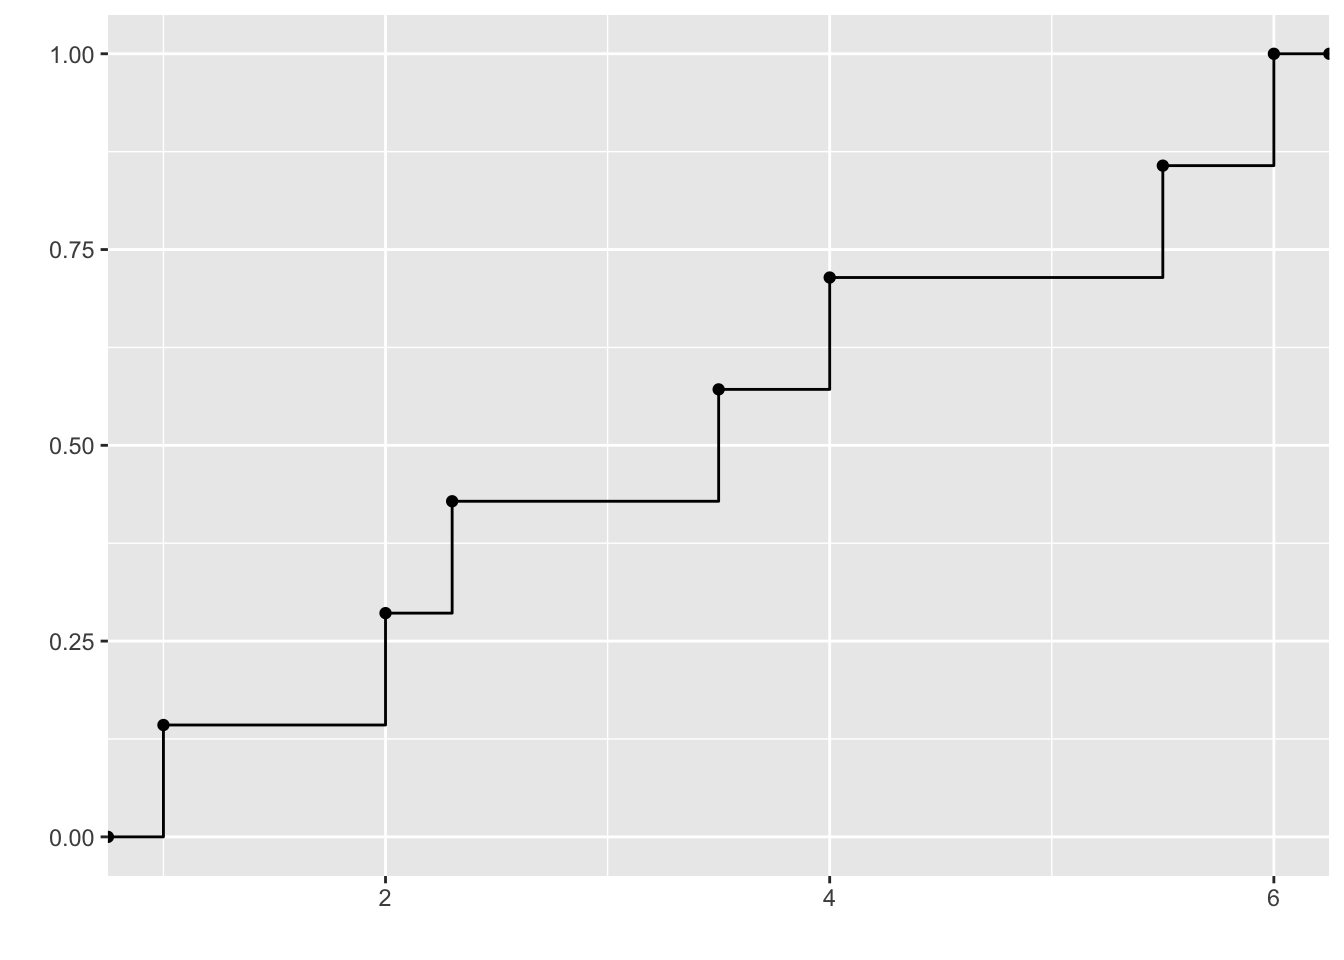
\includegraphics{Bookdown-poly_files/figure-latex/fremp-1.pdf}
\caption{\label{fig:fremp}\label{fremp} Fonction de répartition empirique pour l'échantillon observé \emph{(2, 3.5, 1, 4, 2.3, 6, 5.5)}}
\end{figure}

Rappelons quelques propriétés de la fonction de répartition empirique.

\begin{proposition}
\protect\hypertarget{prp:unlabeled-div-16}{}\label{prp:unlabeled-div-16}

Propriétés de la fonction \(\hat{F}_n(.)\)

\begin{itemize}
\tightlist
\item
  \(\hat{F}_n\) est croissante, continue à droite, \(\underset{t\rightarrow -\infty}{\lim}\hat{F}_n(t)=0\), \(\underset{t\rightarrow +\infty}{\lim}\hat F_n(t)=1\).
\item
  Pour tout \(t\in\mathbb{R}\), \(n \hat{F}_n(t)\) suit une loi binomiale de paramètre \((n, F(t))\).
\item
  Pour tout \(t\in\mathbb{R}\), \(\hat{F}_n(t)\) est un estimateur sans biais de \(F(t)\).
\item
  Pour tout \(t\in\mathbb{R}\)
  \[ \mbox{Var}(\hat{F}_n(t))=\frac{F(t)(1-F(t))}{n} \underset{n\rightarrow +\infty}{\longrightarrow} 0.\]
\item
  Pour tout \(t\in\mathbb{R}\),~\(\hat{F}_n(t) \underset{n\rightarrow+\infty}{\stackrel{\mathbb{P}}{\longrightarrow}}F(t)\)
\item
  On déduit du TLC que pour tout \(t\in\mathbb{R}\) tel que \(F(t)(1-F(t))\neq 0\),
  \[\sqrt{n} (\hat F_n(t)-F(t)) \underset{n\rightarrow+\infty}{\stackrel{\mathcal L}{\longrightarrow}} \mathcal{N} (0, F(t)(1-F(t))).\]
\item
  Glivenko-Cantelli (admis)
  \[
  \underset{t\in\mathbb{R}}{\sup}\  | \hat F_n(t) - F(t) | \underset{n \rightarrow +\infty}{\stackrel{p.s}{\longrightarrow}} 0.
  \]
\end{itemize}

\end{proposition}

\hypertarget{test-de-kolmogorov-de-comparaison-ou-daduxe9quation}{%
\section{Test de Kolmogorov de comparaison ou d'adéquation}\label{test-de-kolmogorov-de-comparaison-ou-daduxe9quation}}

Soit \(X_1, \ldots , X_n\) des v.a.r i.i.d. de même loi que \(X\), de fonction de répartition \(F\) supposée continue. On se donne une fonction de répartition \(F_0\) supposée continue sur \(\mathbb{R}\) et \(Y_0\) une v.a.r de fonction de répartition \(F_0\).

On souhaite construire un test de \(\mathcal{H}_0\): ``\(X\) et \(Y_0\) ont la même loi (\(F=F_0\))'' contre :

\begin{itemize}
\tightlist
\item
  \(\mathcal{H}_1\) : \(X\) et \(Y_0\) ne suivent pas la même loi (\(F\neq F_0\))
\item
  \(\mathcal{H}_1^{+}\) : \(X\) a tendance à prendre des valeurs plus petites que \(Y_0\) (\(F \geq F_0\))
\item
  \(\mathcal{H}_1^{-}\) : \(X\) a tendance à prendre des valeurs plus grandes que \(Y_0\) (\(F \leq F_0\))
\end{itemize}

\begin{figure}
\centering
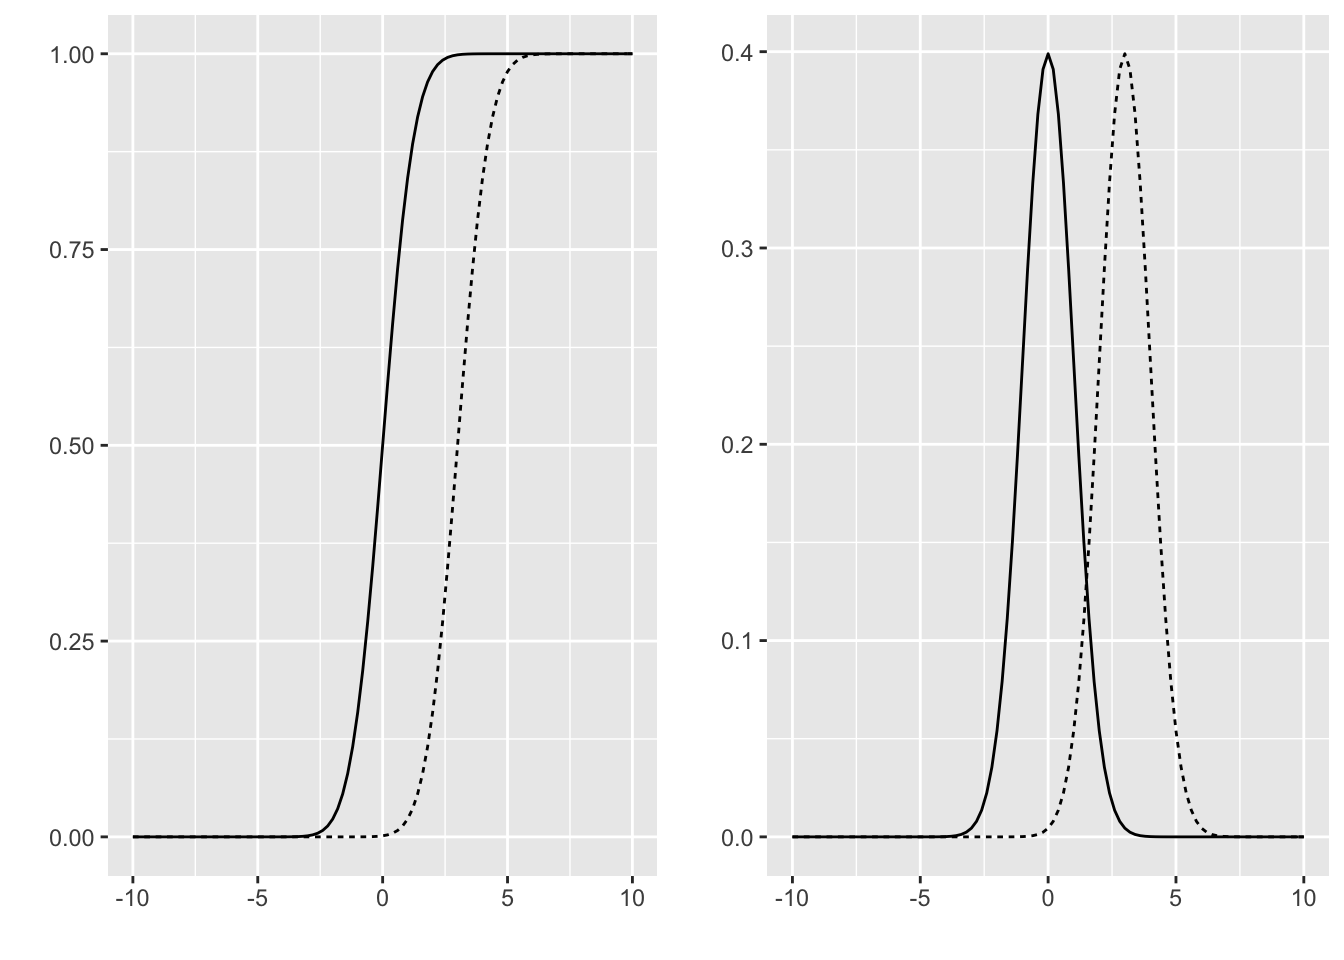
\includegraphics{Bookdown-poly_files/figure-latex/IllustHyp-1.pdf}
\caption{\label{fig:IllustHyp}\label{IllustHyp} Fonction de répartition (à gauche) et densité (à droite) pour la loi N(0,1) et N(3,1)}
\end{figure}

\begin{example}
\protect\hypertarget{exm:unlabeled-div-17}{}\label{exm:unlabeled-div-17}

On mesure les durées de vie de 20 ampoules d'un même type. Les résultats, en heures, sont :
673, 389, 1832, 570, 522, 2694, 3683, 644, 1531, 2916.\\
Est-ce que l'on peut affirmer, au risque 5\(\%\), que la durée de vie d'une ampoule de ce type ne suit pas la loi exponentielle \(\mathcal E(1/1500)\) ?\\
On modélise donc la durée de vie de la \(i\)ème ampoule par \(X_i\), \(F\) est sa fonction de répartition inconnue et \(F_0\) est la fonction de répartition de la loi \(\mathcal E(1/1500)\).

\end{example}

L'idée du test de Kolmogorov est d'estimer la fonction de répartition inconnue \(F\) par la fonction de répartition empirique \(\hat F_n\) de l'échantillon \((X_1,\ldots,X_n)\) et de comparer cette fonction de répartition empirique avec la fonction de répartition donnée \(F_0\).

\begin{definition}
\protect\hypertarget{def:unlabeled-div-18}{}\label{def:unlabeled-div-18}

Pour tester \(\mathcal{H}_0\) contre \(\mathcal{H}_1\), le \textbf{test de Kolmogorov} est fondé sur la statistique de test
\[D_n=\sup_{t \in \mathbb{R}} | \hat F_n(t)-F_0(t)|.\]
La région de rejet au niveau \(\alpha\) est alors de la forme \(\mathcal{R}_{\alpha}=\{D_n \geq d_{n,1-\alpha}\}\).

\end{definition}

\begin{proposition}
\protect\hypertarget{prp:unlabeled-div-19}{}\label{prp:unlabeled-div-19}

Propriétés de la statistique \(D_n\)

\begin{itemize}
\tightlist
\item
  La loi de \(D_n\) sous l'hypothèse \(H_0\) (\(F=F_0\)) est indépendante de \(F_0\).
\item
  Comme \(\hat F_n\) est une fonction en escalier et que \(F_0\) est croissante, l'écart maximal entre \(\hat F_n\) et \(F_0\) est atteint en l'un des sauts de \(\hat F_n\). Ainsi, avec
  \(X_{(1)}\leq \ldots \leq X_{(n)}\) l'échantillon ordonné, \(X_{(0)}=-\infty\) et \(X_{(n+1)}=+\infty\), on obtient que
  \[
    D_n=\max_{i=0,\ldots, n}\left\{\max \left( \left|\frac{i}{n}-F_0(X_{(i)})\right|; \left|\frac{i}{n}-F_0(X_{(i+1)})\right| \right)\right\},
  \]
  ce qui permet de calculer facilement \(D_n\).
\end{itemize}

\end{proposition}

\begin{remark}

La loi de \(D_n\) sous \(H_0\) est tabulée. On trouve dans les tables les quantiles \(d_{n,1-\alpha}\) tels que
\[\mathbb{P}_{H_0} (D_n  \geq d_{n,1-\alpha})\leq \alpha,\]
(en étant le plus proche possible de \(\alpha\)). Ces tables sont obtenues à partir de simulations de \(D_n\), sous l'hypothèse que les \(X_i\) sont i.i.d. de loi uniforme sur \([0,1]\) (\(F_0=\mathbb{1}_{[0,1]}\)). Si la loi de \(D_n\) dépendait de \(F_0\), il faudrait construire une table pour chaque loi \(F_0\).

\end{remark}

\begin{proposition}
\protect\hypertarget{prp:unlabeled-div-21}{}\label{prp:unlabeled-div-21}

De la même façon, pour tester

\begin{itemize}
\tightlist
\item
  \(\mathcal{H}_0 : F=F_0\) contre \(\mathcal{H}^{+} : F \geq F_0\), on utilise
  \[D_n^{+}= \sup_{t \in \mathbb{R}} (\hat{F}_n(t)-F_0(t))\]
  et la région de rejet de niveau \(\alpha\) est de la forme \(\mathcal R_\alpha = \{D_n^{+} > d_{n,1-\alpha}^{+}\}\).
\item
  \(\mathcal{H}_0 : F=F_0\) contre \(\mathcal{H}^{-} : F \leq F_0\), on utilise
  \[D_n^{-}= \sup_{t \in \mathbb{R}} (F_0(t) - \hat{F}_n(t))\]
  et la région de rejet de niveau \(\alpha\) est de la forme \(\mathcal R_\alpha = \{D_n^{-} > d_{n,1-\alpha}^{-}\}\).
\end{itemize}

\end{proposition}

\begin{proposition}
\protect\hypertarget{prp:unlabeled-div-22}{}\label{prp:unlabeled-div-22}

(admise)
\[
\begin{array}{l l }
\forall \lambda >0, \ \mathbb{P}_{\mathcal{H}_0}(\sqrt{n} D_n^+ \geq \lambda) \underset{n \rightarrow +\infty}{\longrightarrow}  \exp(-2\lambda^2)  & \mbox{ Smirnov (1942)} \\
\forall \lambda >0, \mathbb{P}_{\mathcal{H}_0}(\sqrt{n} D_n \geq \lambda)  \underset{n \rightarrow +\infty}{\longrightarrow} 2 \sum_{k=1}^{\infty}(-1)^{k+1}\exp(-2k^2 \lambda^2)  & \mbox{ Kolmogorov (1933)} \\
\forall \lambda >0, \ \mathbb{P}_{\mathcal{H}_0}(\sqrt{n} D_n \geq \lambda)\leq 2 \exp(-2\lambda^2)    & \mbox{ Massart (1990) }
\end{array}
\]

\end{proposition}

\begin{example}
\protect\hypertarget{exm:unlabeled-div-23}{}\label{exm:unlabeled-div-23}

Revenons à notre exemple sur la durée de vie des ampoules. La fonction de répartition empirique et la fonction de répartition de la loi \(\mathcal E(1/1500)\) sont représentées sur la Figure \ref{fig:Ampoule}.
On met en place un test de Kolmogorov pour tester
\[
\mathcal{H}_0 : F = F_0 \textrm{ contre } \mathcal{H}_1 : F \neq F_0,
\]
où \(F_0\) est la fonction de répartition de la loi exponentielle \(\mathcal E(1/1500)\), à l'aide de la fonction \texttt{ks.test}. La p-valeur valant \(0.597\), on ne rejette pas l'hypothèse nulle au niveau \(5\%\).\\
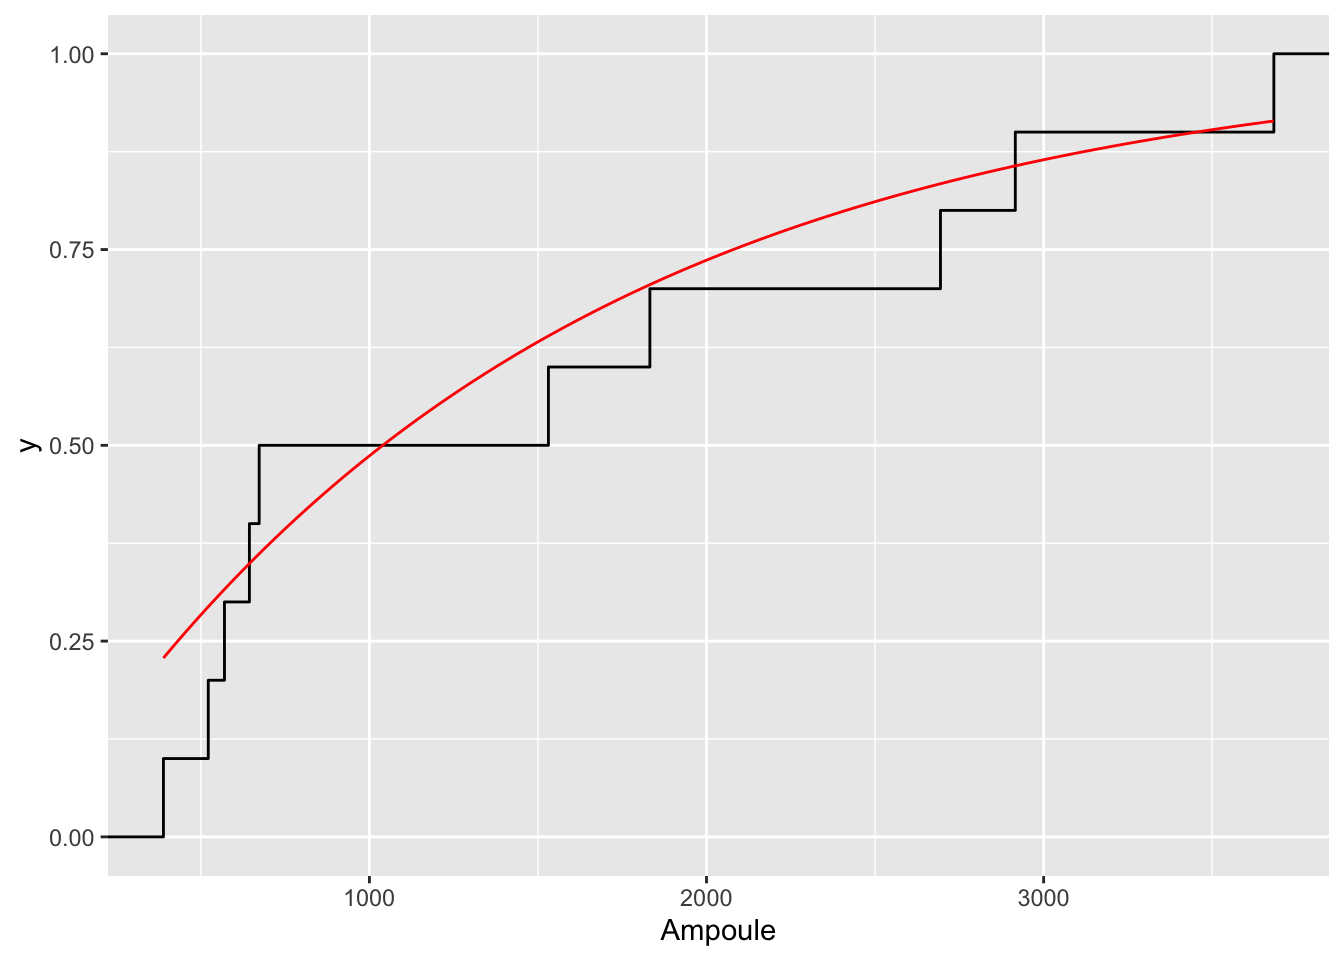
\includegraphics{Bookdown-poly_files/figure-latex/Ampoule-1.pdf}

\begin{Shaded}
\begin{Highlighting}[]
\NormalTok{Ampoule =}\StringTok{ }\KeywordTok{c}\NormalTok{(}\DecValTok{673}\NormalTok{, }\DecValTok{389}\NormalTok{, }\DecValTok{1832}\NormalTok{, }\DecValTok{570}\NormalTok{, }\DecValTok{522}\NormalTok{, }\DecValTok{2694}\NormalTok{, }\DecValTok{3683}\NormalTok{, }\DecValTok{644}\NormalTok{, }\DecValTok{1531}\NormalTok{, }\DecValTok{2916}\NormalTok{) }
\KeywordTok{ks.test}\NormalTok{(Ampoule,pexp,}\DecValTok{1}\OperatorTok{/}\DecValTok{1500}\NormalTok{,}\DataTypeTok{alternative=}\StringTok{"two.sided"}\NormalTok{)}
\end{Highlighting}
\end{Shaded}

\begin{verbatim}

    One-sample Kolmogorov-Smirnov test

data:  Ampoule
D = 0.22843, p-value = 0.597
alternative hypothesis: two-sided
\end{verbatim}

\end{example}

\hypertarget{tests-de-comparaison-de-deux-uxe9chantillons}{%
\section{Tests de comparaison de deux échantillons}\label{tests-de-comparaison-de-deux-uxe9chantillons}}

On considère deux échantillons indépendants

\begin{itemize}
\tightlist
\item
  \(X_1,\ldots, X_n\) i.i.d. de fonction de répartition \(F\)
\item
  \(Y_1, \ldots, Y_m\) i.i.d. de fonction de répartition \(G\).
\end{itemize}

On note \(N=n+m\).

Dans le cas de deux échantillons gaussiens (\(F\) correspond à une loi normale \(\mathcal{N}(m_0, \sigma^2)\) et \(G\) à la loi \(\mathcal{N}(m_1, \sigma^2)\)), on peut utiliser un test de Student pour tester \(\mathcal{H}_0\): \(F=G\) contre \(\mathcal{H}_1\): \(F \neq G\). Nous nous plaçons ici dans un cadre non paramétrique, les lois des variables \(X_i\) et \(Y_j\) ne sont pas supposées connues.

\hypertarget{tests-de-kolmogorov-smirnov}{%
\subsection{Tests de Kolmogorov-Smirnov}\label{tests-de-kolmogorov-smirnov}}

Dans cette section, on souhaite tester \(\mathcal{H}_0\): \(F=G\) contre \(\mathcal{H}_1\): \(F \neq G\). On note \(\hat F_n\) la fonction de répartition empirique de l'échantillon \((X_1, \ldots, X_n)\) et \(\hat G_m\) celle de l'échantillon \((Y_1, \ldots, Y_m)\).

\begin{definition}
\protect\hypertarget{def:unlabeled-div-24}{}\label{def:unlabeled-div-24}

Le \textbf{test de Kolmogorov-Smirnov} est défini par la statistique de test
\[
    D_{n,m}=\sup_{t \in \mathbb{R}} | \hat F_n(t)- \hat G_m(t)|.
\]
La région de rejet au niveau \(\alpha\) est de la forme \(\mathcal R_{\alpha} = \{ D_{n,m} \geq d_{n,m,1-\alpha} \}\).

\end{definition}

\begin{proposition}
\protect\hypertarget{prp:unlabeled-div-25}{}\label{prp:unlabeled-div-25}

Si \(F\) est continue, la loi de \(D_{n,m}\) sous l'hypothèse nulle \(F=G\) est indépendante de \(F\).
Cette loi est tabulée.

\end{proposition}

\begin{remark}

Pour faire un test unilatéral (\(\mathcal{H}_0\): \(F=G\) contre \(\mathcal{H}_1\): \(F \geq G\)), on utilise la statistique de test
\[ 
    D_{n,m}^+=\sup_{t \in \mathbb{R}} (\hat F_n(t)- \hat G_m(t)).
\]
La région de rejet au niveau \(\alpha\) est de la forme \(\mathcal R_{\alpha} = \{ D^+_{n,m} \geq d^+_{n,m,1-\alpha} \}\).

\end{remark}

\begin{example}
\protect\hypertarget{exm:unlabeled-div-27}{}\label{exm:unlabeled-div-27}

On souhaite comparer deux médicaments pour soulager la douleur post-opératoire. On a
observé 16 patients, dont 8 ont pris le médicament A habituel, et les 8 autres un médicament B
expérimental. Dans le tableau suivant sont reportés les temps (en heures) entre la prise du
médicament et la sensation de soulagement.

\begin{tabular}{c|c}
\hline
médicament A & médicament B\\
\hline
6.8 & 4.4\\
\hline
3.1 & 2.5\\
\hline
5.8 & 2.8\\
\hline
4.5 & 2.1\\
\hline
3.3 & 6.6\\
\hline
4.7 & 1.5\\
\hline
4.2 & 4.8\\
\hline
4.9 & 2.3\\
\hline
\end{tabular}

Les fonctions de répartition empiriques des deux échantillons sont représentées en Figure \ref{fig:medicKS}.

Si on veut tester une différence d'efficacité entre les deux médicaments
\[\mathcal{H}_0: F_A = F_B \textrm{ contre }\mathcal{H}_1: F_B\neq F_A\]

\begin{Shaded}
\begin{Highlighting}[]
\NormalTok{mA =}\StringTok{ }\KeywordTok{c}\NormalTok{(}\FloatTok{6.8}\NormalTok{,}\FloatTok{3.1}\NormalTok{,}\FloatTok{5.8}\NormalTok{,}\FloatTok{4.5}\NormalTok{,}\FloatTok{3.3}\NormalTok{,}\FloatTok{4.7}\NormalTok{,}\FloatTok{4.2}\NormalTok{,}\FloatTok{4.9}\NormalTok{)}
\NormalTok{mB =}\StringTok{ }\KeywordTok{c}\NormalTok{(}\FloatTok{4.4}\NormalTok{,}\FloatTok{2.5}\NormalTok{,}\FloatTok{2.8}\NormalTok{,}\FloatTok{2.1}\NormalTok{,}\FloatTok{6.6}\NormalTok{,}\FloatTok{1.5}\NormalTok{,}\FloatTok{4.8}\NormalTok{,}\FloatTok{2.3}\NormalTok{)}
\KeywordTok{ks.test}\NormalTok{(mB, mA, }\DataTypeTok{alternative=}\StringTok{"two.sided"}\NormalTok{)}
\end{Highlighting}
\end{Shaded}

\begin{verbatim}

    Two-sample Kolmogorov-Smirnov test

data:  mB and mA
D = 0.625, p-value = 0.08702
alternative hypothesis: two-sided
\end{verbatim}

Si on veut tester si le médicament \(B\) est plus efficace que le médicament \(A\) :
\[\mathcal{H}_0: F_A = F_B \textrm{ contre }\mathcal{H}_1: F_B\geq F_A\]

\begin{Shaded}
\begin{Highlighting}[]
\KeywordTok{ks.test}\NormalTok{(mB, mA, }\DataTypeTok{alternative=}\StringTok{"greater"}\NormalTok{)}
\end{Highlighting}
\end{Shaded}

\begin{verbatim}

    Two-sample Kolmogorov-Smirnov test

data:  mB and mA
D^+ = 0.625, p-value = 0.04394
alternative hypothesis: the CDF of x lies above that of y
\end{verbatim}

\begin{figure}
\centering
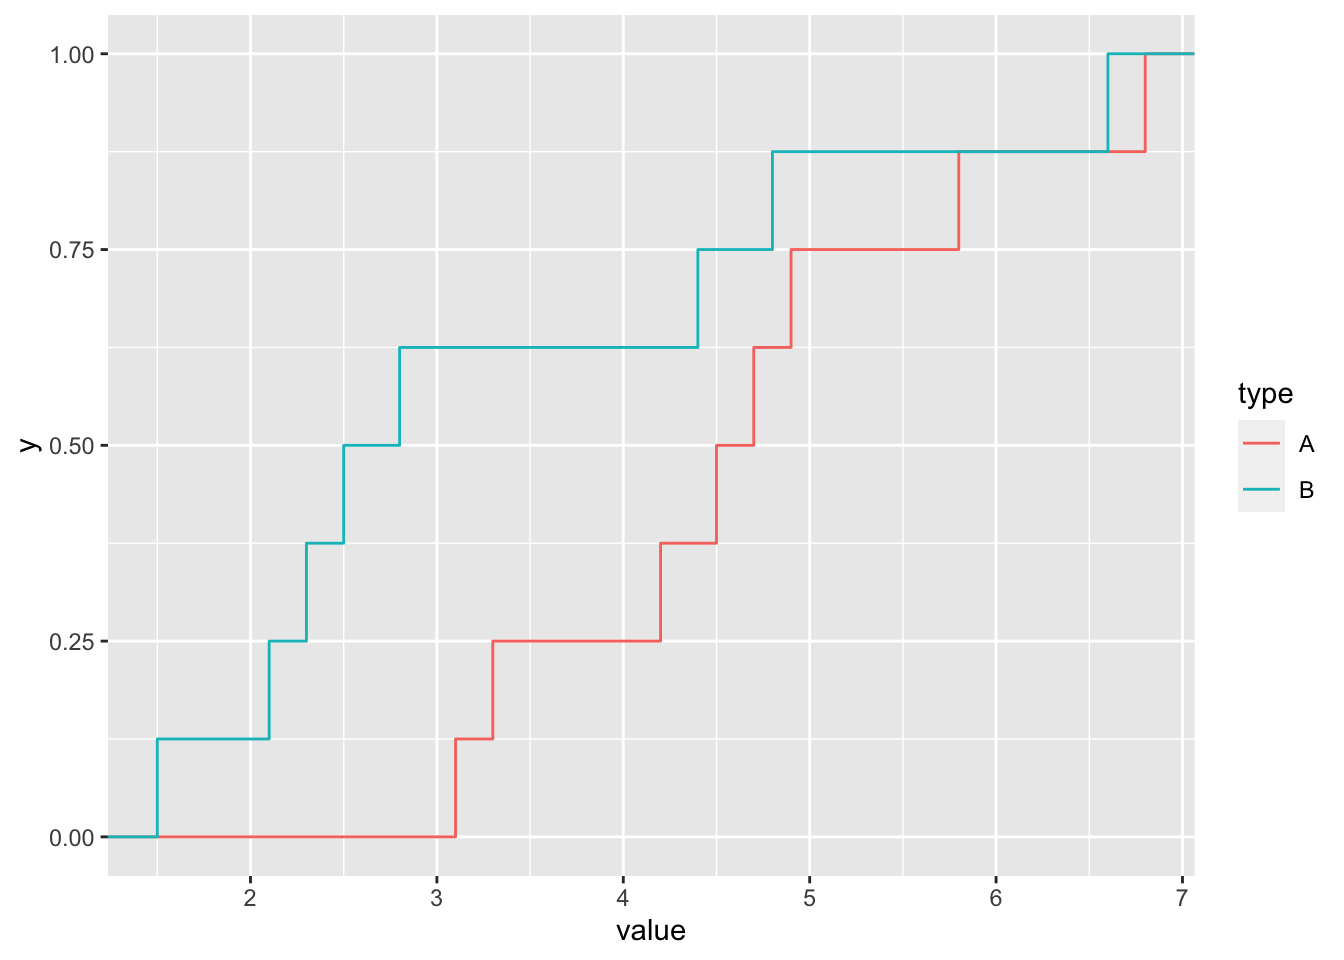
\includegraphics{Bookdown-poly_files/figure-latex/medicKS-1.pdf}
\caption{\label{fig:medicKS}\label{medicKS} Fonction de répartition empirique pour le médicament A en rouge et le médicament B en bleu.}
\end{figure}

\end{example}

\hypertarget{test-de-wilcoxon--mann-whitney}{%
\subsection{Test de Wilcoxon- Mann-Whitney}\label{test-de-wilcoxon--mann-whitney}}

On va s'intéresser dans cette section au test de Mann-Whitney et celui de Wilcoxon (qui sont en fait équivalents) basés sur les rangs.
Pour simplifier la présentation, nous allons supposer dans un premier temps qu'il n'y a pas d'ex-aequo dans les deux échantillons :

\begin{itemize}
\tightlist
\item
  les \(X_i\) sont tous distincts
\item
  les \(Y_j\) sont tous distincts
\item
  les \(X_i\) sont distincts des \(Y_j\) (\(\forall i\neq j, X_i\neq Y_j\)).
\end{itemize}

On reviendra sur le cas des ex-aequo en section \ref{subexaequo}.

\hypertarget{test-de-mann-whitney}{%
\subsubsection{Test de Mann-Whitney}\label{test-de-mann-whitney}}

Supposons que l'on souhaite tester \(\mathcal{H}_0\): \(F=G\) contre \(\mathcal{H}_1\): \(F \geq G\). On suppose que \(F\) et \(G\) sont continues.

Le principe du test de Mann-Whitney consiste à déterminer le nombre de couples \((X_i, Y_j)\) pour lesquels \(Y_j > X_i\). Sous \(\mathcal{H}_1\), pour tout \(t\), \(\mathbb{P}(Y\leq t) \leq P(X\leq t)\) (avec parfois l'inégalité stricte), par conséquent pour tout \(t\), \(\mathbb{P}(Y> t) \geq P(X > t)\) et le nombre de couples \((X_i, Y_j)\) pour lesquels \(Y_j > X_i\) prend des valeurs plus grandes sous \(\mathcal{H}_1\) que sous \(\mathcal{H}_0\).

\begin{proposition}
\protect\hypertarget{prp:unlabeled-div-28}{}\label{prp:unlabeled-div-28}

On appelle \textbf{test de Mann-Whitney} pour \(\mathcal{H}_0\): \(F=G\) contre \(\mathcal{H}_1\): \(F \geq G\) le test défini à partir de la statistique
\[ 
    MW_{X<Y} = \sum_{i=1}^n \sum_{j=1}^m \mathbb{1}_{X_i <Y_j}.
\]
La région de rejet au niveau \(\alpha\) est de la forme \(\mathcal R_{\alpha} = \{MW_{X<Y}\geq u_{(n,m),1-\alpha} \}\).

\end{proposition}

\begin{remark}

La loi de \(MW_{X<Y}\) sous \(\mathcal{H}_0\) peut être établie par récurrence (cf \citet{CaperaaCutsem}, p 126). On note
\[p_{n,m}(k)=\mathbb{P}_{\mathcal{H}_0}( MW_{X<Y} =k) \mbox{ pour } k=0,1, \ldots, mn\]
\[p_{n,0}(k)=p_{0,m}(k)=1  \mbox{ pour } k=0; =0 \mbox{ pour } k\neq 0.\]
Alors pour tout \(k\),
\[ (n+m)p_{n,m}(k)=n p_{n-1,m}(k)+ m p_{n,m-1}(k-n).\]
Cette formule de récurrence permet de calculer la loi de \(MW_{X<Y}\) sous \(\mathcal{H}_0\).

\end{remark}

On peut aussi utiliser un résultat asymptotique.

\begin{theorem}[(Hajek (1968)) (admis)]
\protect\hypertarget{thm:unlabeled-div-30}{}\label{thm:unlabeled-div-30}

Sous \(\mathcal{H}_0\),
\[\frac{MW_{X<Y} -\mathbb{E}_{\mathcal{H}_0}[MW_{X<Y}]}{\sqrt{\mbox{Var}_{\mathcal{H}_0}(MW_{X<Y})}} \stackrel{\mathcal L}{\longrightarrow} \mathcal{N}(0,1)
\mbox{ quand } n\rightarrow +\infty, n/(n+m) \rightarrow \lambda \in ]0,1[.\]

\end{theorem}

On utilise ce résultat en pratique si \(n, m \geq 8\). On a, sous l'hypothèse nulle \(\mathcal{H}_0\) que
\[\mathbb{E}_{\mathcal{H}_0}[MW_{X <Y}]= \frac{mn}{2} \textrm{ et }
\mbox{Var}_{\mathcal{H}_0}(MW_{X < Y})= mn \left(\frac{n+m+1}{12}\right).\]

On peut faire le raisonnement similaire pour tester \(\mathcal{H}_0\): \(F=G\) contre \(\mathcal{H}_1\): \(F \leq G\). Dans ce cas le nombre de couples \((X_i, Y_j)\) pour lesquels \(Y_j < X_i\) prend des valeurs plus grandes sous \(\mathcal{H}_1\) que sous \(\mathcal{H}_0\).

\begin{proposition}
\protect\hypertarget{prp:unlabeled-div-31}{}\label{prp:unlabeled-div-31}

On appelle \textbf{test de Mann-Whitney} pour \(\mathcal{H}_0\): \(F=G\) contre \(\mathcal{H}_1\): \(F \leq G\) le test défini à partir de la statistique
\[ 
MW_{X>Y} = \sum_{i=1}^n \sum_{j=1}^m \mathbb{1}_{X_i >Y_j}.
\]
La région de rejet au niveau \(\alpha\) est de la forme \(\mathcal R_{\alpha} = \{MW_{X>Y}\geq \tilde u_{(n,m),1-\alpha} \}\).

\end{proposition}

La statistique \(MW_{X>Y}\) vérifie des propriétés similaires à celles de \(MW_{X<Y}\) vues précédemment.

Enfin dans le cas d'un test bilatéral de \(\mathcal{H}_0\): \(F=G\) contre \(\mathcal{H}_1\): \(F \neq G\), on combine les deux tests précédents :

\begin{proposition}
\protect\hypertarget{prp:unlabeled-div-32}{}\label{prp:unlabeled-div-32}

On appelle \textbf{test de Mann-Whitney} pour \(\mathcal{H}_0\): \(F=G\) contre \(\mathcal{H}_1\): \(F \neq G\) le test défini à partir de la statistique
\[ 
MW_{X,Y} = max(MW_{X<Y},MW_{X>Y}).
\]
La région de rejet au niveau \(\alpha\) est de la forme \(\mathcal R_{\alpha} = \{MW_{X,Y}\geq v_{(n,m),1-\alpha} \}\).

\end{proposition}

\hypertarget{test-de-wilcoxon}{%
\subsubsection{Test de Wilcoxon}\label{test-de-wilcoxon}}

Revenons au test de \(\mathcal{H}_0\): \(F=G\) contre \(\mathcal{H}_1\): \(F \geq G\). Il existe une autre forme équivalente du test de Mann-Whitney, appelée test de la somme des rangs de Wilcoxon.

Soit \(Z = (Z_1, \ldots, Z_n,Z_{n+1}, \ldots, Z_N)=(X_1, \ldots,X_n,Y_1,\ldots, Y_m)\) l'échantillon complet. On définit \((R_1,\ldots,R_m)\) où \(R_j\) est le rang de \(Y_j\) dans l'échantillon complet ordonné \(Z_{(.)}\) :
\[ R_j=\sum_{k=1}^N \mathbb{1}_{Z_k < Y_j}+1.\]

\begin{proposition}
\protect\hypertarget{prp:unlabeled-div-33}{}\label{prp:unlabeled-div-33}

La statistique de Wilcoxon consiste à calculer la somme des rangs des individus du deuxième échantillon :
\[W_{Y}=\sum_{j=1}^m R_j.\]
Comme on a la relation
\[MW_{X<Y}=  W_{Y} - \frac{m(m+1)}{2},\]
les deux statistiques conduisent au même test.

\end{proposition}

De façon similaire, on peut construire la statistique de test de Wilcoxon \(W_{X}\) (somme des rangs des \(X_i\) dans \(Z\)) liée à la statistique de test \(MW_{X>Y}\) pour tester \(\mathcal{H}_0\): \(F=G\) contre \(\mathcal{H}_1\): \(F \leq G\).

On peut remarquer que
\[
W_X + W_Y = \sum_{k=1}^{n+m} k = \frac{N (N+1)}{2}. 
\]

\begin{example}
\protect\hypertarget{exm:unlabeled-div-34}{}\label{exm:unlabeled-div-34}

On reprend l'exemple des médicaments. On veut tester si le médicament \(B\) est plus efficace que le \(A\) (\(\mathcal{H}_0: F_A=F_B\) contre \(\mathcal{H}_1: F_B \geq F_A\)). On a alors l'échantillon complet ordonné observé

\begin{eqnarray*}
z_{(.)} &=& (1.5, 2.1, 2.3, 2.5, 2.8, 3.1, 3.3, 4.2, 4.4, 4.5, 4.7, 4.8, 4.9, 5.8, 6.6, 6.8)\\
& = & {\scriptsize (mB_6, mB_4, mB_8, mB_2, mB_3, mA_2,mA_5,mA_7,mB_1,mA_4,mA_6,mB_7,mA_8,mA_3,mB_5,mA_1)}
\end{eqnarray*}

Les rangs observés pour les valeurs de B valent donc
\[R_1=9,R_2=4,R_3=5,R_4=2,R_5=15,R_6=1, R_7=12, R_8=3\]
ce qui donne \(W_B=51\) et \(W_A=(16\times 17)/2 - 51 = 85\).

On a également que
\begin{eqnarray*}
MW_{B<A}&=&\sum_{i=1}^8\sum_{j=1}^8 \mathbb{1}_{B_i < A_j}\\ 
&=& 5+ 5+5+6+6+7+7+8 = 49 = W_A - (8 \times 9) /2
\end{eqnarray*}

et

\begin{eqnarray*}
MW_{B>A} &=& \sum_{i=1}^8\sum_{j=1}^8 \mathbb{1}_{B_i > A_j} \\
&=& 3+3+3+2+2+1+1+0=15 = W_B - (8 \times 9) /2. 
\end{eqnarray*}

\begin{Shaded}
\begin{Highlighting}[]
\KeywordTok{wilcox.test}\NormalTok{(mB,mA,}\DataTypeTok{alternative=}\StringTok{"less"}\NormalTok{)}
\end{Highlighting}
\end{Shaded}

\begin{verbatim}

    Wilcoxon rank sum exact test

data:  mB and mA
W = 15, p-value = 0.04149
alternative hypothesis: true location shift is less than 0
\end{verbatim}

\end{example}

\hypertarget{subexaequo}{%
\subsubsection{Traitement des ex-aequos}\label{subexaequo}}

Nous avons supposé les lois continues, donc la probabilité d'avoir des ex-aequos est nulle. En pratique, soit parce que les lois ne sont pas continues, soit parce qu'on a des mesures arrondies, on peut avoir des ex-aequos.
Dans ce cas, on peut considérer les statistiques de test de Mann-Whitney suivantes :
\[ 
    \tilde{MW}_{X<Y} = \sum_{i=1}^n \sum_{j=1}^m \left\{\mathbb{1}_{X_i <Y_j} + \frac 1 2 \mathbb{1}_{X_i =Y_j} \right\}
\]
et
\[ 
    \tilde{MW}_{X>Y} = \sum_{i=1}^n \sum_{j=1}^m \left\{\mathbb{1}_{X_i >Y_j} + \frac 1 2 \mathbb{1}_{X_i =Y_j} \right\}
\]
respectivement. On peut remarquer que \(\tilde{MW}_{X<Y} +\tilde{MW}_{X>Y} =nm\).

Pour le test de Wilcoxon, on utilise les rangs moyens : le rang de tous les éléments d'un groupe d'ex-aequos est la moyenne des rangs des éléments du groupe. On corrige ainsi les \(R_j\) définis précédemment.

\begin{example}
\protect\hypertarget{exm:unlabeled-div-35}{}\label{exm:unlabeled-div-35}

On considère les valeurs observées suivantes pour les deux échantillons :
\[
\underline{x} = (5,3,6,8,1,6) \textrm { avec } n=6
\textrm{ et }
\underline{y} = (5,7,9,5,2) \textrm { avec } m=5.
\]
On obtient alors le tableau des valeurs ordonnées et rangs suivant :

\begin{longtable}[]{@{}llllllllllll@{}}
\toprule
\endhead
\(x_{(.)}\) & 1 & & 3 & & 5 & & 6 & 6 & & 8 &\tabularnewline
\(y_{(.)}\) & & 2 & & 5 & & 5 & & & 7 & & 9\tabularnewline
\(\tilde R_i\) & 1 & & 3 & & 5 & & 7.5 & 7.5 & & 10 &\tabularnewline
\(\tilde R_j\) & & & 2 & & 5 & & 5 & & 9 & & 11\tabularnewline
\bottomrule
\end{longtable}

Ainsi
\[\left(\tilde MW_{X<Y} \right)^{obs} = 1 + (2+\frac 1 2) + (2+\frac 1 2) +5+6=17,\]
\[\left(\tilde W_Y\right)^{obs} = \sum_{j=1}^{5} \tilde R_j = 2+5+5+9+11=32\]
et on retrouve bien que \(\left(\tilde MW_{X<Y} \right)^{obs} =\tilde W_Y^{obs} - \frac{5\times 6}{2}.\)

\end{example}

\hypertarget{test-de-la-muxe9diane}{%
\subsection{Test de la médiane}\label{test-de-la-muxe9diane}}

On veut tester \(\mathcal{H}_0\): \(F=G\) contre \(\mathcal{H}_1\): \(F \geq G\) et on suppose que \(F\) et \(G\) sont continues.
Le principe du test de la médiane consiste à déterminer le nombre de variables du deuxième échantillon qui sont supérieures à la médiane de l'ensemble des observations.

\begin{definition}
\protect\hypertarget{def:unlabeled-div-36}{}\label{def:unlabeled-div-36}

Le \textbf{test de la médiane} est défini à partir de la statistique
\[ M_{X,Y}= \frac1m \sum_{j=1}^m \mathbb{1}_{R_j >\frac{N+1}{2}}.\]
La région de rejet au niveau \(\alpha\) est de la forme \(\mathcal R_\alpha = \{M_{X,Y} \geq m_{n,m,1-\alpha}\}\).

\end{definition}

\begin{example}
\protect\hypertarget{exm:unlabeled-div-37}{}\label{exm:unlabeled-div-37}

Test de localisation.

\(X_1, \ldots, X_n\) sont i.i.d. de fonction de répartition \(F\) et \(Y_1, \ldots, Y_m\) sont i.i.d. de fonction de répartition \(G=F(.-\mu)\). Par exemple, on étudie la pression artérielle de patients soumis à un traitement contre l'hypertension \((Y_j)\), et on les compare à des patients non traités \((X_i)\). Supposons qu'après traitement, la loi de la pression artérielle est translatée de \(\mu\). Le traitement est efficace si \(\mu <0\), il est inefficace si \(\mu=0\).

\end{example}

\textbf{Loi de \(M_{X,Y}\) sous \(\mathcal{H}_0\) :}

\begin{itemize}
\tightlist
\item
  Si \(N\) pair,\\
  \[
  \forall k\in \left\{ \max(0, m - \frac N 2),\ldots,\min(m, \frac N 2)\right\}, \mathbb{P}_{\mathcal{H}_0}(m M_{X,Y}=k)=\frac{C_m^k C_{N-m}^{N/2-k}}{C_{N}^{N/2}}.
  \]
  Donc \(n M_{X,Y}\) suit une loi hypergéométrique \(\mathcal{H}(N,\frac N 2, m)\).
\end{itemize}

On en déduit que \(\mathbb{E}_{\mathcal{H}_0}[M_{X,Y}] = \frac 1 2\) et \(\mbox{Var}_{\mathcal{H}_0}(M_{X,Y}) = \frac{n}{4m(N-1)}\).

\begin{itemize}
\tightlist
\item
  Si \(N\) est impair,\\
  \[
  \forall k\in \left\{ \max(0,m- \frac{N+1}{ 2}),\ldots,\min(m, \frac{N-1}{ 2}) \right\}, \mathbb{P}_{\mathcal{H}_0}(m M_{X,Y}=k)=\frac{C_m^k C_{N-m}^{\frac{N-1}{2}-k}}{C_{N}^{\frac{N-1}{2}}}.
  \]
  Donc \(n M_{X,Y}\) suit une loi hypergéométrique \(\mathcal{H}(N,\frac{N-1}{2}, m)\).
\end{itemize}

On en déduit que \(\mathbb{E}_{\mathcal{H}_0}[M_{X,Y}] = \frac{N-1}{2N}\) et \(\mbox{Var}_{\mathcal{H}_0}(M_{X,Y}) = \frac{n(N+1)}{4mN^2}\).

La connaissance de la loi de \(M_{X,Y}\) sous \(\mathcal{H}_0\) permet de déterminer la région de rejet du test. Pour \(n,m \geq 30\), on peut approximer la loi de \(M_{X,Y}\) sous \(\mathcal{H}_0\) par la loi \(\mathcal{N}(\mathbb{E}_{\mathcal{H}_0}[M_{X,Y}],\mbox{Var}_{\mathcal{H}_0}(M_{X,Y}))\).

\hypertarget{tests-de-normalituxe9}{%
\section{Tests de normalité}\label{tests-de-normalituxe9}}

Dans cette section, on considère un \(n\)-échantillon \((X_1,\ldots,X_n)\) de fonction de répartition \(F\). On note \(\hat F_n\) la fonction de répartition empirique associée à cet échantillon.

Pour illustrer les différentes méthodes, nous allons considérer les trois échantillons de taille \(n=200\) suivants :

\begin{itemize}
\tightlist
\item
  \emph{Ech1} : un échantillon simulé selon la loi \(\mathcal N(2,1)\)
\item
  \emph{Ech2} : un échantillon simulé selon la loi uniforme sur l'intervalle \([2,4]\)
\item
  \emph{Ech3} : un échantillon simulé selon la loi de Cauchy de paramètre 1
\end{itemize}

\begin{Shaded}
\begin{Highlighting}[]
\NormalTok{n=}\DecValTok{200}
\NormalTok{Ech1=}\KeywordTok{rnorm}\NormalTok{(n,}\DecValTok{2}\NormalTok{,}\DecValTok{1}\NormalTok{)}
\NormalTok{Ech2=}\KeywordTok{runif}\NormalTok{(n,}\DataTypeTok{min=}\DecValTok{2}\NormalTok{,}\DataTypeTok{max=}\DecValTok{4}\NormalTok{)}
\NormalTok{Ech3=}\KeywordTok{rcauchy}\NormalTok{(n)}
\end{Highlighting}
\end{Shaded}

\hypertarget{muxe9thode-graphique-droite-de-henry}{%
\subsection{Méthode graphique : droite de Henry}\label{muxe9thode-graphique-droite-de-henry}}

La méthode de la droite de Henry, aussi appelée ``Normal Probability Plot'' ou''Q-Q Plot'', consiste à représenter les points \((X_{(i)}, \Phi^{-1}\circ \hat{F}_n(X_{(i)}))\), où \(X_{(1)} \leq \ldots \leq X_{(n)}\) est l'échantillon ordonné et
\(\Phi\) représente la fonction de répartition de la loi \(\mathcal{N}(0,1)\). Notons que \(\hat F_n(X_{(i)})=i/n\).
Sous l'hypothèse que les \(X_i\) sont i.i.d. de loi normale, les points \((X_{(i)}, \Phi^{-1}\circ \hat F_n(X_{(i)}))\) sont pratiquement alignés. Le Q-Q plot pour les trois échantillons simulés est donné en Figure \ref{fig:QQplot}.

\begin{figure}
\centering
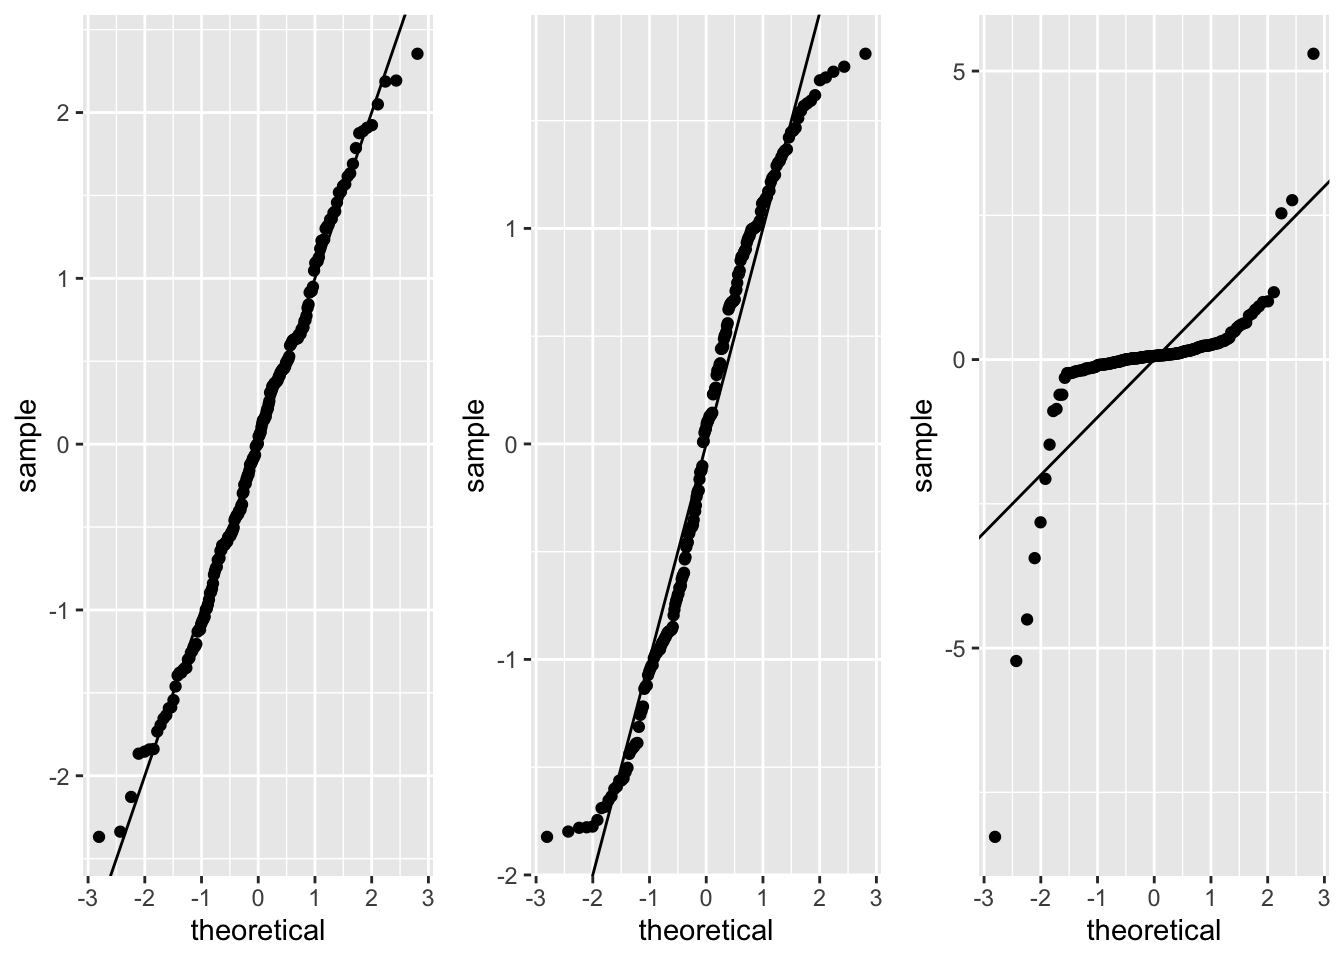
\includegraphics{Bookdown-poly_files/figure-latex/QQplot-1.pdf}
\caption{\label{fig:QQplot}\label{QQplot} Q-Q plot pour les 3 échantillons (N(2,1) à gauche, U({[}2,4{]}) au centre, et C(1) à droite)}
\end{figure}

\hypertarget{test-de-normalituxe9-de-kolmogorov-smirnov-de-lilliefors}{%
\subsection{Test de normalité de Kolmogorov-Smirnov (de Lilliefors)}\label{test-de-normalituxe9-de-kolmogorov-smirnov-de-lilliefors}}

On souhaite tester l'hypothèse \(\mathcal{H}_0\) : ``les \(X_i\) suivent une loi normale'', contre l'hypothèse \(\mathcal{H}_1\) : ``les \(X_i\) ne suivent pas une loi normale''. On note

\[
\bar{X}=\frac1n \sum_{i=1}^n X_i, \ S^2=\frac1{n-1}  \sum_{i=1}^n (X_i-\bar{X})^2.
\]

\begin{definition}
\protect\hypertarget{def:unlabeled-div-38}{}\label{def:unlabeled-div-38}

Le \textbf{test de normalité de Kolmogorov} est fondé sur la statistique de test
\[ 
D\mathcal{N}_n=\sup_{t \in \mathbb{R}}| \hat F_n(t)-\Phi(t; \bar{X},S^2)|
\]
où \(\Phi(. ; \bar{X},S^2)\) est la fonction de répartition de la loi normale \(\mathcal{N}(\bar{X},S^2)\).
La région de rejet au niveau \(\alpha\) est de la forme \(\mathcal R_\alpha = \{ D\mathcal{N}_n > d_{n,1-\alpha}\}\).

\end{definition}

\begin{proposition}
\protect\hypertarget{prp:unlabeled-div-39}{}\label{prp:unlabeled-div-39}

Sous l'hypothèse \(\mathcal{H}_0\), i.e les \(X_i\) suivent une loi normale \(\mathcal{N}(\mu, \sigma^2)\), la loi de \(D\mathcal{N}_n\) ne dépend pas des paramètres inconnus \((\mu, \sigma^2)\). Il s'agit de la loi de
\[
KS\mathcal{N}_n = \underset{t\in\mathbb{R}}{\sup}\ \left|  \hat{\Phi}_n(t) - \Phi\left(\frac{t - \hat\mu_{\mathcal{Z}}}{S_{\mathcal{Z}}}\right)  \right|
\]
où \(\mathcal{Z}=(Z_1,\ldots,Z_n)\) i.i.d de loi \(\mathcal{N}(0,1)\), \(\hat\Phi_n\) la fonction de répartition empirique de \(\mathcal{Z}\), \(\hat\mu_{\mathcal{Z}}\) la moyenne empirique et \(S^2_{\mathcal{Z}}\) la variance empirique de \(\mathcal{Z}\).

\end{proposition}

La loi de \(D\mathcal{N}_n\) est tabulée (on peut par exemple la simuler avec \(\mu=0\) et \(\sigma^2=1\) pour en estimer les quantiles).

On applique le test de normalité de Kolmogorov-Smirnov sur les trois échantillons simulés :

\begin{Shaded}
\begin{Highlighting}[]
\KeywordTok{library}\NormalTok{(nortest)}
\KeywordTok{lillie.test}\NormalTok{(Ech1)}
\end{Highlighting}
\end{Shaded}

\begin{verbatim}

    Lilliefors (Kolmogorov-Smirnov) normality test

data:  Ech1
D = 0.041892, p-value = 0.532
\end{verbatim}

\begin{Shaded}
\begin{Highlighting}[]
\KeywordTok{lillie.test}\NormalTok{(Ech2)}
\end{Highlighting}
\end{Shaded}

\begin{verbatim}

    Lilliefors (Kolmogorov-Smirnov) normality test

data:  Ech2
D = 0.083624, p-value = 0.001691
\end{verbatim}

\begin{Shaded}
\begin{Highlighting}[]
\KeywordTok{lillie.test}\NormalTok{(Ech3)}
\end{Highlighting}
\end{Shaded}

\begin{verbatim}

    Lilliefors (Kolmogorov-Smirnov) normality test

data:  Ech3
D = 0.34735, p-value < 2.2e-16
\end{verbatim}

\hypertarget{test-de-shapiro-wilk}{%
\subsection{Test de Shapiro-Wilk}\label{test-de-shapiro-wilk}}

Il s'agit d'un test basé sur les \(L\)-statistiques (combinaison linéaire des statistiques d'ordre), qui se base sur une comparaison de la variance empirique avec un estimateur de la variance des \(X_i\) qui a de bonnes propriétés sous l'hypothèse de normalité.

\hypertarget{estimation-de-la-moyenne-et-de-la-variance-uxe0-laide-des-statistiques-dordre-pour-des-lois-symuxe9triques}{%
\subsubsection{Estimation de la moyenne et de la variance à l'aide des statistiques d'ordre pour des lois symétriques}\label{estimation-de-la-moyenne-et-de-la-variance-uxe0-laide-des-statistiques-dordre-pour-des-lois-symuxe9triques}}

Soit \(X_1, \ldots, X_n\) i.i.d. On note \(\mu=\mathbb{E}[X_i]\) et \(\sigma^2=\mbox{Var}(X_i)\). La loi de
\(Y_i=(X_i-\mu)/\sigma\) est supposée symétrique (ce qui signifie que \(-Y_i\) a même loi que \(Y_i\)). On note \((X_{(1)}, \ldots, X_{(n)})\) l'échantillon des \(X_i\) ordonné :
\(X_{(1)} \leq \ldots \leq X_{(n)}\). On note \((Y_{(1)}, \ldots, Y_{(n)})\) l'échantillon des \(Y_i\) ordonné. On a
\[Y_{(i)}=(X_{(i)}-\mu)/\sigma.\]
Pour \(i, j \in \{1, \ldots,n\}\), on note
\(\alpha_i=\mathbb{E}[Y_{(i)}]\) et \(B_{i,j}=\mbox{Cov}(Y_{(i)},Y_{(j)}).\)
On a alors
\[X_{(i)}= \mu+\alpha_i \sigma +\varepsilon_i,\]
avec \(\mathbb{E}[\varepsilon_i]=0\). Les \(\varepsilon_i\) ne sont pas indépendantes. La matrice de variance-covariance du vecteur \(\varepsilon=(\varepsilon_1, \ldots, \varepsilon_n)'\) est \(\sigma^2 B\). On note \(1_n\) et \(\alpha\) les vecteurs de \(\mathbb{R}^n\) définis par
\[1_n=\left( \begin{array}{c}  1\\ 1\\ .\\ .\\ 1\end{array} \right), \quad \alpha=\left(\begin{array}{c}  \alpha_1\\ \alpha_2\\ .\\ .\\ \alpha_n \end{array}\right).\]
On note \(A\) la matrice de taille \((n,2)\) définie par \(A=(1_n, \alpha)\). Enfin, on note
\(X_{(.)}=(X_{(1)}, \ldots, X_{(n)})'\) et \(\varepsilon=(\varepsilon_1, \ldots, \varepsilon_n)'\). On a la relation
\[X_{(.)}= A \left( \begin{array}{c} \mu \\ \sigma \end{array}\right) + \varepsilon.\]
L'estimateur des moindres carrés pondérés de \((\mu, \sigma)\) est obtenu en minimisant en les paramètres \((\mu, \sigma)\) le critère :
\[\left( X_{(.)}- A \left( \begin{array}{c} \mu \\ \sigma \end{array}\right)\right)' B^{-1} \left( X_{(.)}- A \left(\begin{array}{c} \mu \\ \sigma\end{array}\right)\right).\]
On obtient comme solution de ce système
\[\left( \begin{array}{c} \hat{\mu}_n \\ \hat{\sigma}_n \end{array}\right)= (A'B^{-1} A)^{-1} A'B^{-1} X_{(.)}.\]
(cf cours sur le modèle linéaire)

\[A'B^{-1} A =  \left( \begin{array}{c c } 1_n'B^{-1} 1_n & 1_n'B^{-1} \alpha \\ \alpha' B^{-1} 1_n & \alpha' B^{-1} \alpha \end{array}\right).\]

\begin{lemma}
\protect\hypertarget{lem:unlabeled-div-40}{}\label{lem:unlabeled-div-40}

Lorsque la loi des \(Y_i\) est symétrique, \(1_n'B^{-1} \alpha =0\) , la matrice \(A'B^{-1} A\) est donc diagonale.

\end{lemma}

Il en résulte que
\[\hat{\mu}_n= \frac{ 1_n'B^{-1} X_{(.)}}{ 1_n'B^{-1} 1_n},\quad \hat{\sigma}_n= \frac{ \alpha'B^{-1} X_{(.)}}{ \alpha'B^{-1} \alpha}.\]
On peut montrer que, si la loi des \(Y_i\) n'est pas symétrique, \(\hat{\sigma}_n\) sous-estime \(\sigma\).

\hypertarget{procuxe9dure-de-test}{%
\subsubsection{Procédure de test}\label{procuxe9dure-de-test}}

\begin{definition}
\protect\hypertarget{def:unlabeled-div-41}{}\label{def:unlabeled-div-41}

Soit \(Y_1, \ldots Y_n\) i.i.d. de loi \(\mathcal{N}(0,1)\) et \(Y_{(1)} \leq \ldots \leq Y_{(n)}\) l'échantillon ordonné.
Soit \(\alpha=(\mathbb{E}[Y_{(1)}], \ldots\mathbb{E}[Y_{(n)}] )'\). Soit \(B\) la matrice de covariance du vecteur \((Y_{(1)},\ldots , Y_{(n)})\).
Le \textbf{test de Shapiro-Wilk} pour tester l'hypothèse de normalité des \(X_i\) est basé sur la statistique de test :
\[ 
    SW_n=\frac{\hat{\sigma}_n^2 (\alpha' B^{-1} \alpha)^2}{\sum_{i=1}^n (X_i-\bar{X}_n)^2 (\alpha' B^{-2} \alpha)}.
\]
On peut l'écrire sous la forme
\[SW_n= \frac{\left(\sum_{i=1}^n a_i X_{(i)}\right)^2}{ \sum_{i=1}^n (X_i-\bar{X}_n)^2},\]
avec
\[(a_1, \ldots,a_n)=\frac{\alpha' B^{-1}}{(\alpha' B^{-1}B^{-1}\alpha)^{1/2}}.\]
La région de rejet est de la forme \(\{SW_n \leq c_{n, \alpha}\}\).

\end{definition}

Les \(a_i\) sont tabulés, ce qui permet de calculer facilement \(SW_n\), les quantiles \(c_{n,\alpha}\) sont également tabulés. On peut interpréter \(SW_n\) comme une mesure de corrélation (au carré) entre les données ordonnées et les statistiques d'ordre d'une loi normale.

Le test de Shapiro-Wilk est ici appliqué sur les trois échantillons simulés :

\begin{Shaded}
\begin{Highlighting}[]
\KeywordTok{shapiro.test}\NormalTok{(Ech1)}
\end{Highlighting}
\end{Shaded}

\begin{verbatim}

    Shapiro-Wilk normality test

data:  Ech1
W = 0.99268, p-value = 0.4201
\end{verbatim}

\begin{Shaded}
\begin{Highlighting}[]
\KeywordTok{shapiro.test}\NormalTok{(Ech2)}
\end{Highlighting}
\end{Shaded}

\begin{verbatim}

    Shapiro-Wilk normality test

data:  Ech2
W = 0.95826, p-value = 1.289e-05
\end{verbatim}

\begin{Shaded}
\begin{Highlighting}[]
\KeywordTok{shapiro.test}\NormalTok{(Ech3)}
\end{Highlighting}
\end{Shaded}

\begin{verbatim}

    Shapiro-Wilk normality test

data:  Ech3
W = 0.45775, p-value < 2.2e-16
\end{verbatim}

\hypertarget{tests-du-khi-deux}{%
\chapter{Tests du khi-deux}\label{tests-du-khi-deux}}

\begin{quote}
Les slides associés à ce chapitre sont disponibles \href{image/SlidesTestsPart2.pdf}{ici}
\end{quote}

La famille des tests du khi-deux regroupe des tests d'objectifs variés (ajustement, indépendance, homogénéité, \ldots)
mais qui ont en commun de mesurer l'écart à l'hypothèse nulle via une ``divergence du khi-deux'' et dont les statistiques de test associées suivent asymptotiquement une loi du khi-deux.
Les tests du khi-deux sont valables pour l'étude de données qualitatives (ou discrètes) à support fini. Cependant, en pratique, ces tests sont aussi appliqués à des données discrètes à support infini ou continues après regroupement en classes.

\hypertarget{test-dajustement-du-khi-deux}{%
\section{Test d'ajustement du khi-deux}\label{test-dajustement-du-khi-deux}}

\hypertarget{objectif-et-principe-du-test}{%
\subsection{Objectif et principe du test}\label{objectif-et-principe-du-test}}

Soit \(X\) une variable aléatoire qualitative ou quantitative discrète à \(K>1\) modalités \(\{a_1,\ldots,a_K\}\), de loi
\(\boldsymbol{\pi}=(\pi_1,\ldots,\pi_K)\) inconnue, où
\[
\pi_k = \mathbb{P}(X=a_k)>0,\ \forall k\in\{1,\ldots,K\}.
\]
On dispose d'un \(n\)-échantillon \((X_1, \ldots X_n)\) de même loi que \(X\). On se donne par ailleurs une loi de probabilité \(\mathcal L_0\) sur \(\{a_1,\ldots,a_K\}\) connue caractérisée par \(\mathbf{p}^0=(p_1^0,\ldots,p_K^0)\) tels que
\[
\forall k,\ p_k^0\in]0,1[ \textrm{ et } \sum_{k=1}^K p_k^0 =1.
\]

On souhaite tester : \(\mathcal{H}_0 : X \sim \mathcal L^0\) contre \(\mathcal{H}_1\) : \(X\) ne suit pas la loi \(\mathcal L^0\).
On peut donc retraduire ces hypothèses de test par
\[
\mathcal{H}_0 : \forall k,\ \pi_k = p_k^0 \textrm{ contre } \mathcal{H}_1 : \exists k,\ \pi_k \neq p_k^0.
\]

Une idée naturelle consiste à estimer la loi de probabilité \(\boldsymbol{\pi}\) de X à l'aide de l'échantillon \((X_1,\ldots,X_n)\) et de comparer cet estimateur avec la loi \(\mathbf{p}^0\). On va donc noter \(N_k= \sum_{i=1}^n \mathbb{1}_{X_i = a_k}\) le nombre de fois que l'on obtient la valeur \(a_k\) dans l'échantillon et on estime \(\pi_k\) par \(\hat{\pi}_k = \frac{N_k}{n}\). On considère alors la statistique
\[
T_{n}= n \sum_{k=1}^K \frac{\left(\hat{\pi}_k - p_k^0\right)^2}{p_k^0} = \sum_{k=1}^K \frac{\left(N_k - n p_k^0\right)^2}{n p_k^0}.
\]
Cette statistique est appelée divergence du khi-deux entre les lois \(\hat{\boldsymbol{\pi}}\) et \(\mathbf{p}^0\). Elle mesure la ``distance'' entre les proportions observées et les proportions théoriques sous \(\mathcal{H}_0\). Mais ce n'est pas une distance car il n'y a pas la propriété de symétrie.

\hypertarget{lien-avec-la-loi-multinomiale}{%
\subsection{Lien avec la loi multinomiale}\label{lien-avec-la-loi-multinomiale}}

\begin{proposition}
\protect\hypertarget{prp:unlabeled-div-42}{}\label{prp:unlabeled-div-42}

La v.a. \(N=(N_{1},\ldots,N_{K})'\) suit une loi multinomiale
\(\mathcal{M}(n,\boldsymbol{\pi})\) sur \(\mathbb{N}^K\), c'est-à-dire que pour tout \((n_1,\ldots,n_K)\in \mathbb{N}^K\) on a
\[
\mathbb{P}(N_{1}=n_1,\ldots,N_{K}=n_K)=\left\{
  \begin{array}{cl}
\frac{n!}{n_1!\ldots n_K!} \pi_1^{n_1}\ldots \pi_K^{n_K}& \ \mbox{ si } \sum_{k=1}^K n_k=n\\
\\
0 &  \ \mbox{ sinon. }
  \end{array}
\right.
\]

\end{proposition}

Ainsi les hypothèses du test peuvent se traduire par
\[
\mathcal{H}_0 : N \sim \mathcal M (n,\mathbf{p}^0) \textrm{ contre } \mathcal{H}_1 : N \textrm{ ne suit pas } \mathcal M(n,\mathbf{p}^0).
\]

\begin{proposition}
\protect\hypertarget{prp:unlabeled-div-43}{}\label{prp:unlabeled-div-43}

Soit \(\sqrt{\boldsymbol{\pi}}=\left(\sqrt{\pi_1},\ldots,\sqrt{\pi_K}\right)'\). On a
\[Y_n=\left(\frac{N_{1}-n \pi_1}{\sqrt{n \pi_1}},\ldots,\frac{N_{K}-n \pi_K}{\sqrt{n \pi_K}}\right) \underset{n\rightarrow +\infty}{\stackrel{\mathcal L}{\longrightarrow}} \mathcal{N}_K\left(0,\Gamma\right),\]
où \(\Gamma= I_K - (\sqrt{\boldsymbol{\pi}}) (\sqrt{\boldsymbol{\pi}})'\) est la matrice de projection orthogonale sur \(\mbox{Vect}(\sqrt{\boldsymbol{\pi}})^{\perp}\).

\end{proposition}

Sous l'hypothèse que \(X_1,\ldots, X_n\) sont i.i.d. de loi \(\boldsymbol{\pi}=(\pi_1,\ldots,\pi_K)\),
\[Z_n=\sum_{k=1}^K \frac{\left(N_{k}-n \pi_k\right)^2}{n \pi_k} \underset{n\rightarrow +\infty}{\stackrel{\mathcal L}{\longrightarrow}} \chi^2(K-1).\]

\hypertarget{procuxe9dure-de-test-1}{%
\subsection{Procédure de test}\label{procuxe9dure-de-test-1}}

On est maintenant en mesure de définir la procédure de test.

\begin{proposition}
\protect\hypertarget{prp:unlabeled-div-44}{}\label{prp:unlabeled-div-44}

Le test d'ajustement du \(\chi^2\) consiste à rejeter l'hypothèse nulle
\(\boldsymbol{\pi}= \mathbf{p}^0\) au niveau \(\alpha\) si
\[T_{n}= \sum_{k=1}^K \frac{\left(N_{k}-n p^0_k\right)^2}{n p^0_k} >x_{K-1,1-\alpha}\]
où \(x_{K-1,1-\alpha}\) est le \(1-\alpha\) quantile d'un \(\chi^2\) à \(K-1\) degrés de liberté.
Ce test est de niveau asymptotique \(\alpha\).

\end{proposition}

On considère en pratique que l'approximation de la loi de \(T_n\)
sous l'hypothèse nulle par une loi du \(\chi^2\) à \(K-1\) degrés de liberté est bonne
dès lors que \(n p^0_k\geq 5\) pour tout \(k\). Lorsque ce n'est pas le cas, on regroupe des classes jusqu'à ce que ces conditions
soient vérifiées. Mais lorsqu'on regroupe des modalités, la région de rejet change car la loi limite dépend du nombres de modalités.

Que peut-on dire de la puissance du test?

On peut remarquer que
\[
\frac{T_n}{n}\geq \| N/n -  \mathbf{p}^0\|^2 \stackrel{p.s}{\longrightarrow} \|\boldsymbol{\pi} -  \mathbf{p}^0\|^2
\]
par la loi des grands nombres et donc \(T_n \stackrel{p.s}{\longrightarrow} +\infty\). La puissance du test
tend donc vers 1 quand \(n\) tend vers \(+\infty\).

\hypertarget{exemple-de-mendel}{%
\subsection{Exemple de Mendel}\label{exemple-de-mendel}}

Chez les pois, le caractère couleur est codé par un gène présentant deux formes allèles J et v correspondant aux couleurs jaune et vert. Le jaune est dominant et le vert récessif. Le caractère de forme, rond ou ridé, est porté par un autre gène à deux allèles R (dominant) et r (récessif). On croise 2 populations (pures) de pois: l'une jaune et ronde, l'autre verte et
ridée. Selon la prédiction de Mendel, au bout de 2 croisements, la proportion de pois

\begin{itemize}
\tightlist
\item
  {[}JR{]} jaunes et ronds est \(9/16\)
\item
  {[}Jr{]} jaunes et ridés est \(3/16\)
\item
  {[}vR{]} verts et ronds est \(3/16\)
\item
  {[}vr{]} verts et ridés est \(1/16\)
\end{itemize}

Dans ses expériences, Mendel a obtenu les résultats suivants :
\(N_{JR}=315\), \(N_{Jr}=101\), \(N_{vR}=108\), \(N_{vr}=32\). Ici \(K=4\) et l'on
obtient que \((T_n)^{obs}=0.47\) et \(x_{3,0.95}=7.82\). On accepte
donc très largement l'hypothèse de Mendel.

\begin{Shaded}
\begin{Highlighting}[]
\NormalTok{Nk=}\KeywordTok{c}\NormalTok{(}\DecValTok{315}\NormalTok{,}\DecValTok{101}\NormalTok{,}\DecValTok{108}\NormalTok{,}\DecValTok{32}\NormalTok{)}
\NormalTok{n =}\StringTok{ }\KeywordTok{sum}\NormalTok{(Nk)}
\NormalTok{ptheo =}\StringTok{ }\KeywordTok{c}\NormalTok{(}\DecValTok{9}\NormalTok{,}\DecValTok{3}\NormalTok{,}\DecValTok{3}\NormalTok{,}\DecValTok{1}\NormalTok{)}\OperatorTok{/}\DecValTok{16}
\KeywordTok{chisq.test}\NormalTok{(Nk,}\DataTypeTok{p=}\NormalTok{ptheo) }
\end{Highlighting}
\end{Shaded}

\begin{verbatim}

    Chi-squared test for given probabilities

data:  Nk
X-squared = 0.47002, df = 3, p-value = 0.9254
\end{verbatim}

\begin{Shaded}
\begin{Highlighting}[]
\KeywordTok{sum}\NormalTok{(((Nk }\OperatorTok{-}\StringTok{ }\NormalTok{(n}\OperatorTok{*}\NormalTok{ptheo))}\OperatorTok{^}\DecValTok{2}\NormalTok{) }\OperatorTok{/}\StringTok{ }\NormalTok{(n}\OperatorTok{*}\NormalTok{ptheo)) }
\end{Highlighting}
\end{Shaded}

\begin{verbatim}
[1] 0.470024
\end{verbatim}

\begin{Shaded}
\begin{Highlighting}[]
\KeywordTok{qchisq}\NormalTok{(}\FloatTok{0.95}\NormalTok{,}\DecValTok{3}\NormalTok{)}
\end{Highlighting}
\end{Shaded}

\begin{verbatim}
[1] 7.814728
\end{verbatim}

\hypertarget{test-du-chi2-daduxe9quation-uxe0-une-famille-de-lois}{%
\section{\texorpdfstring{Test du \(\chi^2\) d'adéquation à une famille de lois}{Test du \textbackslash chi\^{}2 d'adéquation à une famille de lois}}\label{test-du-chi2-daduxe9quation-uxe0-une-famille-de-lois}}

\hypertarget{principe-du-test}{%
\subsection{Principe du test}\label{principe-du-test}}

Soit \(\Theta\) un ouvert de \(\mathbb{R}^d\) avec \(1\leq d<K\).
Etant donnée une famille de lois de probabilités \((\mathcal L(\theta))_{\theta\in\Theta}\) définies sur \(\{a_1,\ldots,a_K\}\), on veut tester
\[
\mathcal{H}_0 : \exists \theta\in\Theta,\ X\sim \mathcal L(\theta)
\]
contre
\[
\mathcal{H}_1 : \textrm{la loi de } X \textrm{ n'appartient pas à } (\mathcal L(\theta))_{\theta\in\Theta}.
\]

Les lois \((\mathcal L(\theta))_{\theta\in\Theta}\) sont caractérisées par les vecteurs de probabilités sur \(\{a_1,\ldots,a_K\}\)
\[
\mathcal P(\Theta)=\left\{ \mathbf{p}(\theta)=(p_1(\theta),\ldots,p_K(\theta));\ \theta\in\Theta \right\}.
\]
On souhaite donc tester
\[
\mathcal{H}_0 : \boldsymbol{\pi}\in \mathcal P(\Theta)  \textrm{ contre }   \mathcal{H}_1 : \boldsymbol{\pi}\notin {\mathcal P}(\Theta).
\]

L'idée du test est de remplacer \(\mathbf{p}^0\) dans \(T_n\) par la loi de \(\mathcal P(\Theta)\) ``la plus proche'' de \(\boldsymbol{\pi}\) au vu des données, c'est-à-dire la loi \(\mathbf{p}(\hat\theta)\) où \(\hat\theta\) est l'estimateur du maximum de vraisemblance pour le paramètre \(\theta\) basé sur l'échantillon \((X_1,\ldots,X_n)\) sous \(\mathcal{H}_0\). On considère donc la statistique suivante :
\[
\hat T_n = n \sum_{k=1}^K \frac{\left(\hat{\pi}_k - p_k(\hat\theta)\right)^2}{p_k(\hat\theta)} = \sum_{k=1}^K \frac{\left(N_k - n p_k(\hat\theta)\right)^2}{n p_k(\hat\theta)}.
\]

Or, on a le résultat (admis) suivant :

\begin{theorem}
\protect\hypertarget{thm:unlabeled-div-45}{}\label{thm:unlabeled-div-45}

Supposons que

\begin{itemize}
\tightlist
\item
  Pour tout \(k=1,\ldots,K\), \(\theta\mapsto p_k(\theta)\) est \({\mathcal C}^2\) sur \(\Theta\) et vérifie pour tout \(\theta\in \Theta\),
  \(p_k(\theta)\neq 0\).
\item
  Pour tout \(\theta\in \Theta\), les vecteurs
  \(v_i=\left(\partial_i p_1(\theta), \ldots,\partial_i p_K(\theta)\right))'\) pour
  \(i=1,\ldots, d\) forment une famille libre de \(\mathbb{R}^K\) (bonne
  paramétrisation).
\item
  Pour tout \(\theta\), si \(X_1,\ldots, X_n\) sont i.i.d. de loi \(\mathbf{p}(\theta)\)
  alors l'estimateur du maximum de vraisemblance \(\hat \theta\) est consistant
  vers \(\theta\).
\end{itemize}

Sous ces conditions, si \(X_1,\ldots, X_n\) sont i.i.d. de loi \(\mathbf{p}(\theta)\)
alors
\[
    \hat T_n \underset{n\rightarrow +\infty}{\stackrel{\mathcal L}{\longrightarrow}}\chi^2(K-d-1).
\]

\end{theorem}

On construit le test du \(\chi^2\) d'adéquation à \({\mathcal P}(\Theta)\) de
la manière suivante:

on rejette l'hypothèse nulle si\\
\[\hat T_n= \sum_{k=1}^K \frac{\left(N_k - n p_k(\hat\theta)\right)^2}{n p_k(\hat\theta)} > x_{K-d-1,1-\alpha}.\]
La p-valeur vaut
\[
p( (\hat T_n)^{obs}) = \mathbb{P}_{\mathcal{H}_0}(\hat T_n \geq  (\hat T_n)^{obs}) \underset{n \rightarrow +\infty}{\longrightarrow}    \mathbb{P}( \chi^2(K-d-1) \geq  (\hat T_n)^{obs}). 
\]
Sous l'alternative:\\
\[
\frac{\hat T_n}{n} \geq \rm{d}^2( N/n, {\mathcal P}(\Theta)) \stackrel{p.s}{\longrightarrow} \rm{d}^2 (\boldsymbol{\pi}, {\mathcal P}(\Theta)),
\]
et donc la puissance tend vers 1 dès que
\(\rm{d}^2(\boldsymbol{\pi},{\mathcal P}(\Theta))>0\).

\begin{remark}

Le nombre de degrés de liberté de la loi asymptotique est donné par ``nombre de modalités - 1 - nombre de paramètres à estimer sous \(\mathcal{H}_0\).''

\end{remark}

\hypertarget{exemple}{%
\subsection{Exemple}\label{exemple}}

Pour \(10000\) fratries de \(4\) enfants, on a relevé le nombre de garçons :

\begin{longtable}[]{@{}llllll@{}}
\toprule
\endhead
Nb de garçons \((k)\) & 0 & 1 & 2 & 3 & 4\tabularnewline
Effectifs \((N_k)\) & 572 & 2329 & 3758 & 2632 & 709\tabularnewline
\bottomrule
\end{longtable}

On décide de modéliser les naissances en supposant qu'elles sont indépendantes et que la probabilité d'avoir un garçon vaut \(\theta\in]0,1[\).
On note \(X_i\) le nombre de garçons dans la \(i\)ème fratrie. On souhaite donc tester
\[
\mathcal{H}_0 : X_i \sim \mathcal Bin(4,\theta) \textrm{ contre } \mathcal{H}_1 : X_i \textrm{ ne suit pas une loi } \mathcal Bin(4,\theta), \theta\in]0,1[.
\]
Sous \(\mathcal{H}_0\), l'estimateur du maximum de vraisemblance pour \(\theta\) est donné par \(\hat \theta = \frac{\overline{X}_n}{4}\). On peut alors calculer \(\mathbf{p}(\hat\theta) = (p_0(\hat\theta),\ldots,p_4(\hat\theta))\) avec \(p_k(\hat\theta) = \mathbb{P}( U = k)\) pour \(U\sim \mathcal Bin(4,\hat\theta)\). Sous \(\mathcal{H}_0\), la statistique de test
\[
\hat T_n =  \sum_{k=0}^4 \frac{\left(N_k - n p_k(\hat\theta)\right)^2}{n p_k(\hat\theta)}  \underset{n\rightarrow +\infty}{\stackrel{\mathcal L}{\longrightarrow}}\chi^2(5-1-1) =\chi^2(3).
\]

\begin{Shaded}
\begin{Highlighting}[]
\NormalTok{classes =}\StringTok{ }\KeywordTok{c}\NormalTok{(}\DecValTok{0}\NormalTok{,}\DecValTok{1}\NormalTok{,}\DecValTok{2}\NormalTok{,}\DecValTok{3}\NormalTok{,}\DecValTok{4}\NormalTok{)}
\NormalTok{Nk =}\StringTok{ }\KeywordTok{c}\NormalTok{(}\DecValTok{572}\NormalTok{,}\DecValTok{2329}\NormalTok{,}\DecValTok{3758}\NormalTok{,}\DecValTok{2632}\NormalTok{,}\DecValTok{709}\NormalTok{)}
\NormalTok{n =}\StringTok{ }\KeywordTok{sum}\NormalTok{(Nk)}
\NormalTok{pihat =}\StringTok{ }\NormalTok{Nk }\OperatorTok{/}\StringTok{ }\NormalTok{n}
\NormalTok{thetahat =}\StringTok{ }\KeywordTok{sum}\NormalTok{(Nk }\OperatorTok{*}\StringTok{ }\NormalTok{classes) }\OperatorTok{/}\StringTok{ }\NormalTok{(n}\OperatorTok{*}\DecValTok{4}\NormalTok{)}
\NormalTok{ptheo =}\StringTok{ }\KeywordTok{dbinom}\NormalTok{(}\DecValTok{0}\OperatorTok{:}\DecValTok{4}\NormalTok{,}\DecValTok{4}\NormalTok{,thetahat)}
\NormalTok{Tobs =}\StringTok{ }\KeywordTok{sum}\NormalTok{(((Nk }\OperatorTok{-}\StringTok{ }\NormalTok{(n}\OperatorTok{*}\NormalTok{ptheo))}\OperatorTok{^}\DecValTok{2}\NormalTok{) }\OperatorTok{/}\StringTok{ }\NormalTok{(n}\OperatorTok{*}\NormalTok{ptheo)) }
\KeywordTok{print}\NormalTok{(Tobs)}
\end{Highlighting}
\end{Shaded}

\begin{verbatim}
[1] 0.9882779
\end{verbatim}

\begin{Shaded}
\begin{Highlighting}[]
\NormalTok{val =}\StringTok{ }\KeywordTok{chisq.test}\NormalTok{(Nk,}\DataTypeTok{p=}\NormalTok{ptheo)  }\CommentTok{# Attention aux degrés de liberté ! }
\KeywordTok{print}\NormalTok{(val)}
\end{Highlighting}
\end{Shaded}

\begin{verbatim}

    Chi-squared test for given probabilities

data:  Nk
X-squared = 0.98828, df = 4, p-value = 0.9116
\end{verbatim}

\begin{Shaded}
\begin{Highlighting}[]
\NormalTok{pval =}\StringTok{ }\DecValTok{1} \OperatorTok{-}\StringTok{ }\KeywordTok{pchisq}\NormalTok{(val}\OperatorTok{$}\NormalTok{statistic,}\DecValTok{3}\NormalTok{)}
\KeywordTok{print}\NormalTok{(pval)}
\end{Highlighting}
\end{Shaded}

\begin{verbatim}
X-squared 
0.8040883 
\end{verbatim}

\hypertarget{test-du-chi2-dinduxe9pendance}{%
\section{\texorpdfstring{Test du \(\chi^2\) d'indépendance}{Test du \textbackslash chi\^{}2 d'indépendance}}\label{test-du-chi2-dinduxe9pendance}}

\hypertarget{principe-du-test-1}{%
\subsection{Principe du test}\label{principe-du-test-1}}

Soient \(X\) et \(Y\) deux variables aléatoires admettant un nombre fini de modalités, \(\{a_1,\ldots,a_K\}\) et \(\{b_1,\ldots,b_L\}\) respectivement. On considère \(n\) couples aléatoires \((X_1,Y_1),\ldots,(X_n,Y_n)\) indépendants et de même loi que \((X,Y)\).
On souhaite tester
\[
\mathcal{H}_0 : X \textrm{ et } Y \textrm{ sont indépendantes contre } \mathcal{H}_1 : X \textrm{ et } Y \textrm{ ne sont pas indépendantes}. 
\]

On va ici donner une idée de la construction de la statistique de test. On rappelle tout d'abord que la loi du couple \((X,Y)\) est caractérisée par les probabilités
\[
    \mathbb{P}(X=a_k,Y=b_l) \textrm{ pour tout } k=1,\ldots,K,\ l=1,\ldots,L.
\]
On est sous \(\mathcal{H}_0\) quand \(\forall (k,l),\ \mathbb{P}(X=a_k, Y=b_l) = \mathbb{P}(X=a_k) \mathbb{P}(Y=b_l)\) et sous \(\mathcal{H}_1\) si \(\exists (k,l),\ \mathbb{P}(X=a_k, Y=b_l) \neq \mathbb{P}(X=a_k) \mathbb{P}(Y=b_l)\).

On introduit les variables aléatoires suivantes :

\begin{itemize}
\tightlist
\item
  \(N_{k,l} = \sum_{i=1}^n \mathbb{1}_{X_i = a_k, Y_i = b_l}\)
\item
  \(N_{k,.} = \sum_{i=1}^n \mathbb{1}_{X_i = a_k} = \sum_{l=1}^L N_{k,l}\)
\item
  \(N_{.,l} = \sum_{i=1}^n \mathbb{1}_{Y_i = b_l} = \sum_{k=1}^K N_{k,l}\)
\end{itemize}

On peut alors estimer \(\mathbb{P}(X=a_k, Y=b_l)\) par \(N_{k,l}/n\) et \(\mathbb{P}(X=a_k) \mathbb{P}(Y=b_l)\) par \(N_{k,.} N_{.,l} / n^2\). En reprenant le même raisonnement que dans les sections précédentes, on obtient la statistique de test suivante :
\[
I_n = n \sum_{k=1}^K \sum_{l=1}^L \frac{\left(\frac{N_{k,l}}{n}    -  \frac{N_{k,.} N_{.,l}}{n^2}   \right)^2}{ \frac{N_{k,.} N_{.,l}}{n^2} } = \sum_{k=1}^K \sum_{l=1}^L \frac{\left(N_{k,l}    -  \frac{N_{k,.} N_{.,l}}{n}   \right)^2}{ \frac{N_{k,.} N_{.,l}}{n} }. 
\]

\hypertarget{procuxe9dure-de-test-2}{%
\subsection{Procédure de test}\label{procuxe9dure-de-test-2}}

On suppose que \(\forall k,\ \mathbb{P}(X=a_k)>0\) et \(\forall l,\ \mathbb{P}(Y=b_l)>0\). Alors, sous \(\mathcal{H}_0\),
\[
I_n \underset{n\rightarrow +\infty}{\stackrel{\mathcal L}{\longrightarrow}}\chi^2((K-1)(L-1)).
\]

\begin{remark}

Pour retrouver rapidement le nombre de degrés de liberté, il faut remarquer que le nombre de modalités du couple \((X, Y)\) vaut \(K L\). Et sous \(\mathcal{H}_0\), comme \(\forall (k,l),\ \mathbb{P}(X=a_k, Y=b_l) = \mathbb{P}(X=a_k)\mathbb{P}(Y=b_l)\), il faut estimer les \(\mathbb{P}(X=a_k)\) pour \(k=1,\ldots,K-1\) et les \(\mathbb{P}(Y=b_l)\) pour \(l=1,\ldots, L-1\). Ainsi le nombre de degrés de liberté est \((KL-1) - [(K-1)+(L-1)] = (K-1)(L-1)\).

\end{remark}

\begin{proposition}
\protect\hypertarget{prp:unlabeled-div-48}{}\label{prp:unlabeled-div-48}

Soit \(\alpha\in]0,1[\). Le test de région de rejet
\[
\mathcal R_\alpha = \{ I_n > x_{(K-1)(L-1),1-\alpha} \}
\]
est un test de niveau asymptotique \(\alpha\) pour tester \(\mathcal{H}_0\) contre \(\mathcal{H}_1\).

\end{proposition}

\hypertarget{exemple-1}{%
\subsection{Exemple}\label{exemple-1}}

Une enquête a été réalisée auprès d'un échantillon de \(250\) personnes au sujet de l'abaissement à 16 ans du droit de vote. Les réponses ont été classées suivant le niveau d'instruction des personnes interrogées :

\begin{longtable}[]{@{}llll@{}}
\toprule
Niveau d'instruction & Pour & Contre & \(N_{k.}\)\tabularnewline
\midrule
\endhead
Brevet & 10 & 15 & 25\tabularnewline
Bac & 20 & 85 & 105\tabularnewline
Bac +2 et plus & 20 & 100 & 120\tabularnewline
& & &\tabularnewline
\(N_{.l}\) & 50 & 200 & 250\tabularnewline
\bottomrule
\end{longtable}

Peut-on affirmer, au risque d'erreur de \(5\%\), qu'il existe une relation entre l'opinion d'une personne sur cette question et son niveau d'instruction ?

\begin{Shaded}
\begin{Highlighting}[]
\NormalTok{contingence =}\StringTok{ }\KeywordTok{matrix}\NormalTok{(}\KeywordTok{c}\NormalTok{(}\DecValTok{10}\NormalTok{,}\DecValTok{20}\NormalTok{,}\DecValTok{20}\NormalTok{,}\DecValTok{15}\NormalTok{,}\DecValTok{85}\NormalTok{,}\DecValTok{100}\NormalTok{),}\DataTypeTok{ncol=}\DecValTok{2}\NormalTok{)}
\KeywordTok{chisq.test}\NormalTok{(contingence)}
\end{Highlighting}
\end{Shaded}

\begin{verbatim}

    Pearson's Chi-squared test

data:  contingence
X-squared = 7.1429, df = 2, p-value = 0.02812
\end{verbatim}

\hypertarget{test-dhomoguxe9nuxe9ituxe9}{%
\section{Test d'homogénéité}\label{test-dhomoguxe9nuxe9ituxe9}}

\hypertarget{principe-du-test-2}{%
\subsection{Principe du test}\label{principe-du-test-2}}

Soit \(E_1, \ldots, E_L\) \(L\)-échantillons indépendants de lois discrètes sur le même support \(\{a_1,\ldots,a_K\}\). On note \(\boldsymbol{\pi}_l\) la loi discrète de l'échantillon \(E_l=(X_{l,1},\ldots,X_{l,n_l})\) de taille \(n_l\).
On veut tester
\[
\mathcal{H}_0: \textrm{ les échantillons sont issus de la même loi } (\boldsymbol{\pi}_1=\ldots=\boldsymbol{\pi}_L)
\]
contre
\[
\mathcal{H}_1: \textrm{ les échantillons ne sont pas issus de la même loi } (\exists j\neq l,\ \boldsymbol{\pi}_j \neq \boldsymbol{\pi}_l)
\]

\hypertarget{procuxe9dure-de-test-3}{%
\subsection{Procédure de test}\label{procuxe9dure-de-test-3}}

On note \(N_{k,l} = \sum_{i=1}^{n_l} \mathbb{1}_{X_{l,i} = a_k}\), \(N_{k,.}= \sum_{l=1}^{L} N_{k,l}\) et \(N_{.,l}=\sum_{k=1}^K N_{k,l}=n_\ell\).
On considère alors la statistique de test :
\[
J_n =  \sum_{k=1}^K \sum_{\ell=1}^L \frac{\left(N_{k,l}    -  \frac{N_{k,.} N_{.,l}}{n}   \right)^2}{ \frac{N_{k,.} N_{.,l}}{n} }. 
\]

On suppose que \(\forall k,\forall l, \boldsymbol{\pi}_{l,k}=\mathbb{P}(X_{l,i}=a_k)>0\). Alors, sous \(\mathcal{H}_0\),
\[
J_n \underset{n\rightarrow +\infty}{\stackrel{\mathcal L}{\longrightarrow}}\chi^2((K-1)(L-1)).
\]

\begin{proposition}
\protect\hypertarget{prp:unlabeled-div-49}{}\label{prp:unlabeled-div-49}

Soit \(\alpha\in]0,1[\). Le test de région de rejet
\[
\mathcal R_\alpha = \{ J_n > x_{(K-1)(L-1),1-\alpha} \}
\]
est un test de niveau asymptotique \(\alpha\) pour tester \(\mathcal{H}_0\) contre \(\mathcal{H}_1\).

\end{proposition}

\hypertarget{exemple-2}{%
\subsection{Exemple}\label{exemple-2}}

Dans cet exemple, on souhaite savoir si le taux de participation à un club sportif des élèves de deux collèges \(A\) et \(B\) est identique ou pas.
On a donc deux échantillons \(E_1=(X_{1,1},\ldots,X_{1,n_1})\) et \(E_2=(X_{2,1},\ldots,X_{2,n_2})\) avec
\[
X_{l,i}= \textrm{ participation du } i \textrm{ème élève du collège } l \in \{a_1,a_2\}=\{"oui","non"\}.
\]
On veut tester
\[
\mathcal{H}_0 : \textrm{ les 2 populations sont homogènes (même taux de participation)}
\]
contre
\[
\mathcal{H}_1 : \textrm{ les 2 populations ne sont pas homogènes}.
\]

On a les effectifs observés suivants :

\begin{longtable}[]{@{}lccc@{}}
\toprule
Partic. / Ech & collège A & collège B & \(N_{k,.}\)\tabularnewline
\midrule
\endhead
oui & 12 & 26 & 38\tabularnewline
non & 38 & 34 & 72\tabularnewline
& & &\tabularnewline
\(N_{.,l}\) & 50 & 60 & \(n=110\)\tabularnewline
\bottomrule
\end{longtable}

et les effectifs théoriques sont :

\begin{longtable}[]{@{}ccc@{}}
\toprule
Partic. / Ech & collège A & collège B\tabularnewline
\midrule
\endhead
oui & 17,27 & 20,73\tabularnewline
non & 32,73 & 39,27\tabularnewline
\bottomrule
\end{longtable}

La statistique de test observée vaut donc
\[(J_n)^{obs} = \frac{(12-17,27)^2}{17,27} + \ldots + \frac{(34-39,27)^2}{39,27}=4,504 > x_{1,0.95}=3.84\]
donc on rejette \(\mathcal{H}_0\), le taux de participation à un club sportif est différent entre les deux collèges.

  \bibliography{BiblioTest.bib}

\end{document}
